\documentclass[11pt]{article}
\usepackage[a4paper,margin=25mm,marginparwidth=20mm,marginparsep=10pt]{geometry}
\usepackage{fontspec}
\usepackage{amsmath,amssymb,mathtools}
\usepackage{unicode-math}
\usepackage[normalem]{ulem}
\usepackage{graphicx,xcolor,tikz,tikz-cd}
\usetikzlibrary{calc,decorations.pathmorphing,decorations.pathreplacing,arrows.meta,shapes.geometric}
\newcommand{\scanpage}[1]{\par\medskip\noindent{\footnotesize\textcolor{gray}{[scan #1]}}\par}
\newcommand{\mspage}[1]{{\footnotesize\textcolor{gray}{[p.~#1]}}\ }
\newcommand{\unsure}[1]{{\color{blue}#1}}
\newcommand{\illegible}[1]{\textcolor{red}{[illeg.~#1]}}
\newcommand{\deleted}[1]{{\color{gray}#1}}
\newcommand{\inserted}[1]{{\color{teal}#1}}
\newcommand{\margin}[1]{\ifinner{\footnotesize[#1]}\else\marginpar{\footnotesize #1}\fi}
\newcommand{\diagram}[1]{\ifmmode\vcenter{\hbox{#1}}\else\ifinner #1\else\par\begin{center}#1\end{center}\par\fi\fi}
\let\figure\relax\newcommand{\figure}[1]{\ifmmode\vcenter{\hbox{#1}}\else\ifinner #1\else\par\begin{center}#1\end{center}\par\fi\fi}

\setmathfont{Latin Modern Math}
\usepackage{newunicodechar}
\newfontfamily\cyrfont{DejaVu Serif}[Scale=MatchLowercase]
\let\oldGamma\Gamma\renewcommand\Gamma{\ensuremath{\oldGamma}}
\let\oldsimeq\simeq\renewcommand\simeq{\ensuremath{\oldsimeq}}
\renewcommand\margin[1]{\parbox{120pt}{\footnotesize #1}}
\setbox0=\hbox{test}
\newunicodechar{А}{{\cyrfont\char"0410}}
\newunicodechar{Б}{{\cyrfont\char"0411}}
\newunicodechar{В}{{\cyrfont\char"0412}}
\newunicodechar{Г}{{\cyrfont\char"0413}}
\newunicodechar{Д}{{\cyrfont\char"0414}}
\newunicodechar{Е}{{\cyrfont\char"0415}}
\newunicodechar{Ж}{{\cyrfont\char"0416}}
\newunicodechar{З}{{\cyrfont\char"0417}}
\newunicodechar{И}{{\cyrfont\char"0418}}
\newunicodechar{Й}{{\cyrfont\char"0419}}
\newunicodechar{К}{{\cyrfont\char"041A}}
\newunicodechar{Л}{{\cyrfont\char"041B}}
\newunicodechar{М}{{\cyrfont\char"041C}}
\newunicodechar{Н}{{\cyrfont\char"041D}}
\newunicodechar{О}{{\cyrfont\char"041E}}
\newunicodechar{П}{{\cyrfont\char"041F}}
\newunicodechar{Р}{{\cyrfont\char"0420}}
\newunicodechar{С}{{\cyrfont\char"0421}}
\newunicodechar{Т}{{\cyrfont\char"0422}}
\newunicodechar{У}{{\cyrfont\char"0423}}
\newunicodechar{Ф}{{\cyrfont\char"0424}}
\newunicodechar{Х}{{\cyrfont\char"0425}}
\newunicodechar{Ц}{{\cyrfont\char"0426}}
\newunicodechar{Ч}{{\cyrfont\char"0427}}
\newunicodechar{Ш}{{\cyrfont\char"0428}}
\newunicodechar{Щ}{{\cyrfont\char"0429}}
\newunicodechar{Ъ}{{\cyrfont\char"042A}}
\newunicodechar{Ы}{{\cyrfont\char"042B}}
\newunicodechar{Ь}{{\cyrfont\char"042C}}
\newunicodechar{Э}{{\cyrfont\char"042D}}
\newunicodechar{Ю}{{\cyrfont\char"042E}}
\newunicodechar{Я}{{\cyrfont\char"042F}}
\newunicodechar{а}{{\cyrfont\char"0430}}
\newunicodechar{б}{{\cyrfont\char"0431}}
\newunicodechar{в}{{\cyrfont\char"0432}}
\newunicodechar{г}{{\cyrfont\char"0433}}
\newunicodechar{д}{{\cyrfont\char"0434}}
\newunicodechar{е}{{\cyrfont\char"0435}}
\newunicodechar{ж}{{\cyrfont\char"0436}}
\newunicodechar{з}{{\cyrfont\char"0437}}
\newunicodechar{и}{{\cyrfont\char"0438}}
\newunicodechar{й}{{\cyrfont\char"0439}}
\newunicodechar{к}{{\cyrfont\char"043A}}
\newunicodechar{л}{{\cyrfont\char"043B}}
\newunicodechar{м}{{\cyrfont\char"043C}}
\newunicodechar{н}{{\cyrfont\char"043D}}
\newunicodechar{о}{{\cyrfont\char"043E}}
\newunicodechar{п}{{\cyrfont\char"043F}}
\newunicodechar{р}{{\cyrfont\char"0440}}
\newunicodechar{с}{{\cyrfont\char"0441}}
\newunicodechar{т}{{\cyrfont\char"0442}}
\newunicodechar{у}{{\cyrfont\char"0443}}
\newunicodechar{ф}{{\cyrfont\char"0444}}
\newunicodechar{х}{{\cyrfont\char"0445}}
\newunicodechar{ц}{{\cyrfont\char"0446}}
\newunicodechar{ч}{{\cyrfont\char"0447}}
\newunicodechar{ш}{{\cyrfont\char"0448}}
\newunicodechar{щ}{{\cyrfont\char"0449}}
\newunicodechar{ъ}{{\cyrfont\char"044A}}
\newunicodechar{ы}{{\cyrfont\char"044B}}
\newunicodechar{ь}{{\cyrfont\char"044C}}
\newunicodechar{э}{{\cyrfont\char"044D}}
\newunicodechar{ю}{{\cyrfont\char"044E}}
\newunicodechar{я}{{\cyrfont\char"044F}}
\begin{document}
\typeout{LMSTART 85}
\setbox0=\hbox\bgroup
\begin{tikzcd}[ampersand replacement=\&,column sep=1.2em,row sep=1.7em]
\Pi_{0,3}^{D} \arrow[r] \arrow[ddrr]
\& \Pi_{0,3}^{D}/\uline{\Pi'_{0,3}} \arrow[r,"\sim"]
\& \overbrace{\mathbb Z/6\mathbb Z\times_{\mathbb Z/2\mathbb Z}\mathbb D_3}^{18}
  \arrow[rr,"{\simeq(\mathbb F_3\times\mathbb F_3)\unsure{\rtimes|\cdot}\{1,\sigma\}}"]
  \arrow[dd]
\& \& \mathbb Z/6\mathbb Z \arrow[r]
\& \mathbb Z/2\mathbb Z
\\
\mathrm S\ell(2,\mathbb Z) \arrow[u] \arrow[rrr]
  \arrow[ddrrr]
\& \begin{gathered}\text{sous-groupe}\\
   \text{d'indice }3\text{ de }\Pi_{0,3}\\
   \text{obtenu en}\\
   \text{faisant }\rho_0=\unsure{\rho_1}(=\rho_\infty)\\
   \rho_0^3=1\end{gathered}
\& \& \begin{gathered}\deleted{\unsure{\mathrm S\ell(2,\mathbb Z)/\varepsilon}}\quad\mathcal E^{36}\\
\simeq\mathrm S\ell(2,\mathbb Z/6\mathbb Z)/\bigl(\text{sous-groupe d'ordre }2\bigr)\\
\text{à déterminer}\end{gathered}
\arrow[ul] \arrow[dd] \arrow[r]
\& \deleted{\unsure{\mathbb Z/2\mathbb Z}}\ \mathbb Z/12\mathbb Z
  \arrow[u] \arrow[ur] \arrow[r,no head]
\& \mathbb Z/4\mathbb Z \arrow[u]
\\
\& \widetilde{\mathrm S\ell}(2,\mathbb Z) \arrow[ul] \arrow[rrrr]
\& {}^{6}\mathbb D_3 \arrow[ur,no head]
\& \& \& \mathbb Z \arrow[ul,bend left=16]
\\
\& \& \& \underset{12}{\mathbb D'_3\ \unsure{\sim}}
  \arrow[ul] \arrow[uurr]
\& \&
% five squares carry the word Cart (cartesien) written inside them, not on an arrow
\arrow[from=2-2,to=1-3,phantom,"\mathrm{Cart}"{description}]
\arrow[from=2-4,to=1-5,phantom,"\mathrm{Cart}"{description}]
\arrow[from=2-5,to=1-6,phantom,"\mathrm{Cart}"{description}]
\arrow[from=2-4,to=3-3,phantom,"\mathrm{Cart}"{description}]
\arrow[from=2-2,to=3-3,phantom,"\mathrm{Cart}"{description}]
\end{tikzcd}
\egroup
\typeout{LMWIDTH 85 \the\wd0 HEIGHT \the\ht0 DEPTH \the\dp0}
\typeout{LMSTART 86}
\setbox0=\hbox\bgroup
\begin{tikzcd}[ampersand replacement=\&,column sep=3em,row sep=2em]
\begin{gathered}
\Pi_{0,3}^{D}/\Pi'_{0,3}\simeq
\{\rho,\sigma\mid\rho^3=\sigma^2=(\sigma\rho)^6=1,\
(\sigma\rho)^2\deleted{\text{central}}\inserted{=(\rho\sigma)^2}\}
\qquad18
\end{gathered}
\arrow[d,"{\substack{\rho\mapsto4\ \mathrm{mod}\ 6\\\sigma\mapsto3\ \mathrm{mod}\ 6}}"]
\arrow[dr,"{\substack{\rho\mapsto\rho\\\sigma\mapsto\sigma}}"]
\& \\
\mathbb Z/6\mathbb Z
\& \begin{gathered}\mathbb D_3=\{\rho,\sigma\mid\rho^3=\sigma^{2}\deleted{\unsure{2}}=1,\
\sigma(\rho)=\rho^{-1}\}\!\\
\inserted{\text{i.e. }(\sigma\rho)^2=1}
\end{gathered}
\end{tikzcd}
\egroup
\typeout{LMWIDTH 86 \the\wd0 HEIGHT \the\ht0 DEPTH \the\dp0}
\typeout{LMSTART 87}
\setbox0=\hbox\bgroup
\begin{tikzcd}[ampersand replacement=\&,row sep=1.5em,column sep=3em]
{} \arrow[d] \&
\left\{\begin{array}{rcl}
\rho&\mapsto&\unsure{10|14}\ \mathrm{mod}\ 12\\
\sigma&\mapsto&3\ \mathrm{mod}\ 12\\
\omega&\mapsto&6\ \mathrm{mod}\ 12
\end{array}\right.
\\
\unsure{\leftrightarrows}\ \mathbb Z/12\mathbb Z
\simeq(\mathrm S\ell(2,\mathbb Z))_{\mathrm{ab}} \&
\end{tikzcd}
\egroup
\typeout{LMWIDTH 87 \the\wd0 HEIGHT \the\ht0 DEPTH \the\dp0}
\typeout{LMSTART 88}
\setbox0=\hbox\bgroup
\begin{tikzcd}[ampersand replacement=\&,column sep=1.7em,row sep=1.5em,
execute at end picture={\draw ([xshift=0.4em,yshift=2em]current bounding box.south west)--([xshift=5em,yshift=-6em]current bounding box.north west);}]
\& \& \& \& \& 0 \arrow[dl]
\\
\& \& \deleted{\unsure{(\sigma\rho)^2\omega}}
\& \& \unsure{\mathbb Z/3\mathbb Z}\times_{\mathbb Z/2\mathbb Z}\{0\}
\arrow[d,no head,"\simeq"] \arrow[ddll]
\& 0 \arrow[dl]
\\
\& \& \& \& \mathbb Z/3\mathbb Z \arrow[ddll] \&
\\
\& \begin{array}{|l}\unsure{(\mathbb F_3\times\mathbb F_3)\rtimes\{1,\sigma\}}\simeq\\\sigma\end{array}
\& \mathbb Z/6\mathbb Z\times_{\mathbb Z/2\mathbb Z}\mathbb D_3
\arrow[uu] \arrow[rr,"\mathrm{pr}_1"] \arrow[ddl]
\& \& \mathbb Z/6\mathbb Z \&
\\
\& \& \mathcal E \arrow[u] \arrow[rr] \arrow[ddl]
\& \& \mathbb Z/12\mathbb Z \arrow[u,"\unsure{Can}"'] \&
\\
\& \mathbb D_3 \arrow[dl] \& \mathbb Z/2\mathbb Z \arrow[u] \& \& \&
\\
0 \& \mathbb D'_3 \arrow[u] \arrow[dl]
\& 0 \arrow[u] \& \& \&
\\
0 \& \& \& \& \&
\end{tikzcd}
\egroup
\typeout{LMWIDTH 88 \the\wd0 HEIGHT \the\ht0 DEPTH \the\dp0}
\typeout{LMSTART 89}
\setbox0=\hbox\bgroup
\begin{tikzcd}[ampersand replacement=\&,row sep=1.5em,column sep=4em]
1 \arrow[d] \& \& 0 \arrow[d]
\\
\mathbb Z\widetilde\omega \arrow[d]
\& \widetilde\omega=(1,2n)
\& \mathbb Z \arrow[d,"2n"]
\\
\widetilde\Pi_n^D \arrow[d] \arrow[rr] \& \& \mathbb Z \arrow[d]
\\
\Pi_n^D=\{\rho,\sigma\mid\rho^n=\sigma^2=1\}
\arrow[d] \arrow[rr,Rightarrow]
\& \& (\Pi_n^D)_{\mathrm{ab}}\simeq\mathbb Z/2n\mathbb Z
\\
1 \& \&
\begin{gathered}
\rho\longmapsto(n+1\ \mathrm{mod}\ 2n)=(1-n\ \mathrm{mod}\ 2n)\\
\sigma\longmapsto n\ \mathrm{mod}\ 2n
\end{gathered}
\end{tikzcd}
\egroup
\typeout{LMWIDTH 89 \the\wd0 HEIGHT \the\ht0 DEPTH \the\dp0}
\typeout{LMSTART 90}
\setbox0=\hbox\bgroup
\begin{tikzcd}[ampersand replacement=\&,row sep=large,column sep=small]
\& 1 \& \& 1 \\
\& \mathcal T_{11} \arrow[u] \arrow[r] \& \deleted{\unsure{\mathcal T_{\mathrm{ab}}}} \arrow[r] \& \mathbb Z/12\mathbb Z \arrow[u] \\
\unsure{\widetilde\omega|\bar\omega}=\omega^{2\deleted{\unsure{4}}} \& S\mathcal T_{11} \arrow[u] \arrow[rr] \arrow[ur,phantom,"\deleted{\text{cartésien}}"{description}] \& \& \mathbb Z \arrow[u] \\
\uline{1} \arrow[u] \& \mathbb Z \arrow[u] \arrow[rr,"\mathrm{id}"] \& \& \mathbb Z \arrow[u,"12"] \\
\& 1 \arrow[u] \& \& 1 \arrow[u]
\end{tikzcd}
\egroup
\typeout{LMWIDTH 90 \the\wd0 HEIGHT \the\ht0 DEPTH \the\dp0}
\typeout{LMSTART 91}
\setbox0=\hbox\bgroup
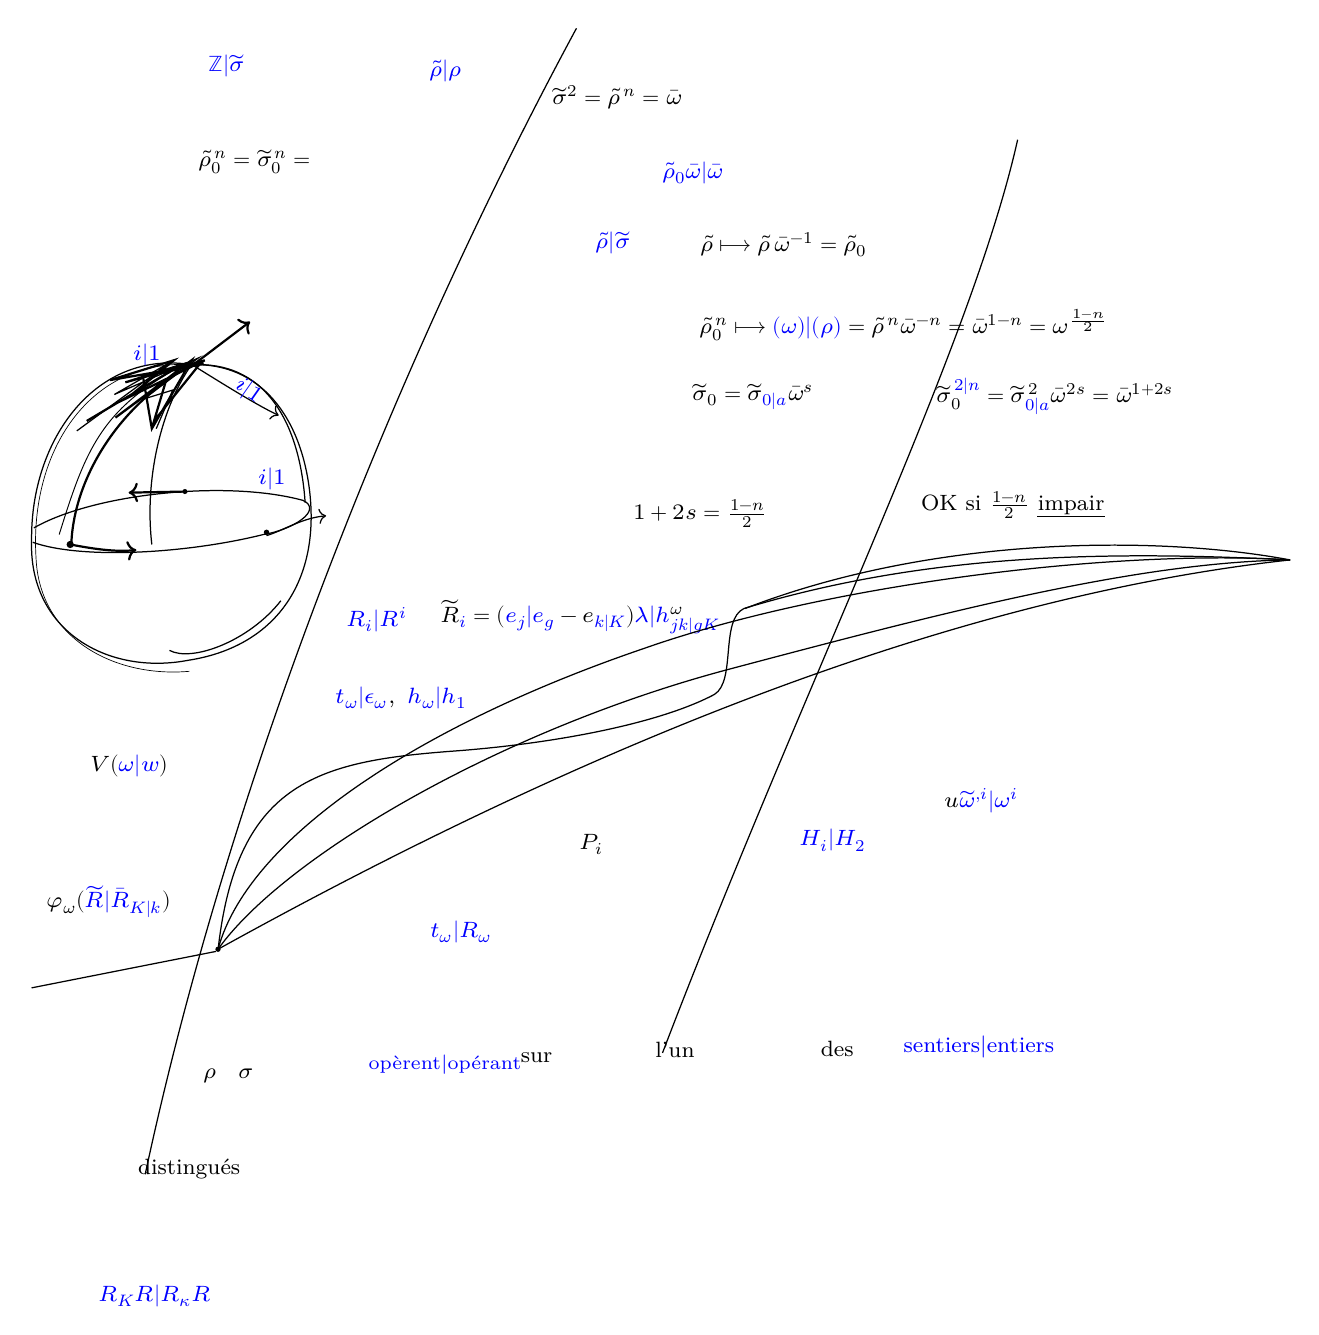
\begin{tikzpicture}[x=.014cm,y=-.014cm,every node/.style={font=\footnotesize,inner sep=0pt},line width=.45pt]
\node[anchor=west] at (385,80) {$\deleted{\unsure{\mathbb Z|\widetilde\sigma}}$};
\node[anchor=west] at (585,85) {$\deleted{\unsure{\widetilde\rho|\rho}}$};
\node[anchor=west] at (376,167) {$\widetilde\rho_0^{\,n}=\widetilde\sigma_0^{\,n}=$};
\node[anchor=west] at (697,109) {$\widetilde\sigma^2=\widetilde\rho^{\,n}=\bar\omega$};
\node[anchor=west] at (796,177) {$\deleted{\unsure{\widetilde\rho_0\bar\omega|\bar\omega}}$};
\node[anchor=west] at (736,241) {$\deleted{\unsure{\widetilde\rho|\widetilde\sigma}}$};
\node[anchor=west] at (831,242) {$\widetilde\rho\longmapsto\widetilde\rho\,\bar\omega^{-1}=\widetilde\rho_0$};
\node[anchor=west] at (830,315) {$\widetilde\rho_0^{\,n}\longmapsto\deleted{\unsure{(\omega)|(\rho)}}=\widetilde\rho^{\,n}\bar\omega^{-n}=\bar\omega^{1-n}=\omega^{\frac{1-n}{2}}$};
\node[anchor=west] at (824,380) {$\widetilde\sigma_0=\widetilde\sigma_{\unsure{0|a}}\bar\omega^s$};
\node[anchor=west] at (1045,380) {$\widetilde\sigma_0^{\,\unsure{2|n}}=\widetilde\sigma_{\unsure{0|a}}^{\,2}\bar\omega^{2s}=\bar\omega^{1+2s}$};
\node[anchor=west] at (770,486) {$1+2s=\frac{1-n}{2}$};
\node[anchor=west] at (1031,478) {OK si $\frac{1-n}{2}$ \uline{impair}};

\draw (328,1085) .. controls (405,726) and (557,346) .. (719,46);
\draw (797,975) .. controls (925,640) and (1077,335) .. (1119,147);

\draw (370,351) .. controls (284,337) and (224,418) .. (225,510) .. controls (222,592) and (294,633) .. (367,619) .. controls (445,607) and (487,549) .. (477,465) .. controls (469,399) and (433,349) .. (370,351);
\draw[line width=.25pt] (371,351) .. controls (277,345) and (223,430) .. (229,526) .. controls (232,599) and (300,635) .. (368,629);
\draw (350,610) .. controls (370,621) and (422,602) .. (451,565);
\draw (227,499) .. controls (281,468) and (401,455) .. (471,474) .. controls (490,483) and (461,501) .. (435,505) .. controls (367,522) and (271,528) .. (226,512);
\draw[line width=.8pt,->] (260,514) .. controls (281,518) and (301,521) .. (320,519);
\draw[line width=.8pt,->] (366,466)--(313,467);
\draw[->] (438,506) .. controls (454,501) and (470,490) .. (492,488);
\fill (260,514) circle[radius=3.3];
\fill (438,503) circle[radius=2.5];
\fill (364,466) circle[radius=2.3];
\draw (334,514) .. controls (327,454) and (343,389) .. (370,351);
\draw[line width=.8pt] (261,514) .. controls (263,455) and (303,388) .. (370,351);
\draw[line width=.35pt] (250,505) .. controls (274,428) and (288,390) .. (365,350);
\draw[line width=.8pt,->] (369,353)--(423,312);
\draw[->] (372,352) .. controls (398,368) and (428,387) .. (449,397);
\draw (377,351) .. controls (437,351) and (468,403) .. (473,476);
\node at (330,342) {$\unsure{i|1}$};
\node[rotate=-35] at (422,375) {$\unsure{i|1}$};
\node at (443,455) {$\unsure{i|1}$};
\draw[line width=.8pt] (275,402)--(361,351)--(310,367)--(382,347)--(312,381)--(354,347)--(296,365)--(377,351)--(336,402)--(347,365)--(301,399)--(370,347)--(334,409)--(326,362)--(381,350);
\draw (266,411)--(352,348)--(300,378)--(376,345)--(327,382)--(353,374)--(338,409);

\node[anchor=west] at (510,582) {$\unsure{R_i|R^i}$};
\node[anchor=west] at (595,580) {$\widetilde R_{\unsure{i}}=(\unsure{e_j|e_g}-e_{\unsure{k|K}})\unsure{\lambda|h}^{\omega}_{\unsure{jk|gK}}$};
\node[anchor=west] at (500,653) {$\unsure{t_\omega|\epsilon_\omega},\ \unsure{h_\omega|h_1}$};
\node[anchor=west] at (278,715) {$V(\unsure{\omega|w})$};
\node[anchor=west] at (238,838) {$\varphi_\omega(\unsure{\widetilde R|\bar R}_{\unsure{K|k}})$};
\node[anchor=west] at (721,786) {$P_i$};
\node[anchor=west] at (586,865) {$\deleted{\unsure{t_\omega|R_\omega}}$};
\node[anchor=west] at (921,782) {$\deleted{\unsure{H_i|H_2}}$};
\node[anchor=west] at (1052,746) {$u\unsure{\widetilde\omega^{,i}|\omega^i}$};

\draw (225,916)--(392,883);
\fill (394,881) circle[radius=2.4];
\draw (394,882) .. controls (411,727) and (487,710) .. (612,701) .. controls (702,694) and (795,676) .. (844,650) .. controls (864,638) and (849,582) .. (871,572) .. controls (1039,521) and (1205,520) .. (1366,528);
\draw (394,881) .. controls (422,778) and (581,676) .. (781,608) .. controls (949,549) and (1211,518) .. (1366,528);
\draw (394,881) .. controls (454,797) and (649,683) .. (854,628) .. controls (1057,574) and (1228,530) .. (1366,528);
\draw (394,881) .. controls (721,700) and (1056,562) .. (1366,528);
\draw (872,572) .. controls (1045,505) and (1249,506) .. (1366,528);

\node[anchor=west] at (380,996) {$\rho\quad\sigma$};
\node[anchor=west,font=\scriptsize] at (530,986) {\unsure{opèrent|opérant}};
\node[anchor=west] at (668,979) {sur};
\node[anchor=west] at (790,972) {l'un};
\node[anchor=west] at (940,971) {des};
\node[anchor=west] at (1015,970) {\unsure{sentiers|entiers}};
\node[anchor=west] at (321,1080) {distingués};
\node[anchor=west] at (285,1195) {$\deleted{\unsure{R_KR|R_\kappa R}}$};
\end{tikzpicture}
\egroup
\typeout{LMWIDTH 91 \the\wd0 HEIGHT \the\ht0 DEPTH \the\dp0}
\typeout{LMSTART 92}
\setbox0=\hbox\bgroup
\begin{tikzcd}[ampersand replacement=\&,column sep=1.6em,row sep=2.8em]
\&\&
\begin{gathered}
\widetilde\rho=(\rho_0,2)=(\rho,2)\\
\widetilde\sigma=(\sigma_0,3)=(\sigma,3)
\end{gathered}
\arrow[d, bend right=20]
\&
\begin{gathered}
\deleted{\unsure{\Pi_{0,3}^{D}}}\\[-2pt]
\inserted{\text{\uline{\unsure{identifié à}}}}\\[-2pt]
\inserted{\unsure{S\mathcal T_{11}\times_{\Pi_{0,3}^{D}}\mathbb Z/12\mathbb Z}}
\end{gathered}
\arrow[d]
\&
\begin{gathered}
\rho_0=(\rho,\dot 2)\\[-2pt]
\unsure{\Pi_{0,3}}\\[-2pt]
\sigma_0=(\sigma,\dot 3)=(\sigma,-1)
\end{gathered}
\arrow[d]
\&\\
\unsure{0|1}\arrow[r,dash]\&
\mathbb Z\arrow[r,dash,"1\unsure{-|\mapsto}\overline\omega=\omega^2"]\arrow[dd,equal]\&
S\mathcal T_{11}\arrow[r,Rightarrow]\arrow[dd,"\substack{\widetilde\rho\mapsto\deleted{\unsure{4}}2\\\widetilde\sigma\mapsto3}"']
\arrow[ddr,phantom,"\text{Cart}"]\&
\mathcal T_{11}\arrow[r,Rightarrow]\arrow[dr,leftrightarrow]\arrow[dd,"\substack{\rho_0\mapsto\dot 2\\\sigma_0\mapsto\dot 3}"']
\&\Pi_{0,3}^{\prime D}\arrow[dr,"\text{can}"]\arrow[dd,"\substack{\rho\mapsto2\\\sigma\mapsto3}"{pos=.25,xshift=2pt}]
\arrow[dl,phantom,"\text{cart}" description]\&\\
\&\&\&{}\&
|[xshift=-3em]|\mathbb D'_3\arrow[r,"\text{cart}"{pos=.75}]\arrow[dd]
\&\mathbb D_3\arrow[dd,"\text{can}"]\\
1\arrow[r,dash]\&\mathbb Z\arrow[r,"12"]\&\mathbb Z\arrow[r,"\text{can}"]\&
\mathbb Z/12\mathbb Z\arrow[r,"\text{can}"]\arrow[dr,"\text{can}"']
\&\mathbb Z/6\mathbb Z\arrow[dr,"\text{can}"]
\arrow[d,phantom,"\text{\uline{Cart}}"'{pos=.25,xshift=-3em}]
\arrow[dr,phantom,"\text{\uline{cart}}"{description,xshift=-1.5em,yshift=.5em}]\&\\
\&\&\&\&\mathbb Z/4\mathbb Z\arrow[r,leftrightarrow,"\text{can}"]\&\mathbb Z/2\mathbb Z
\end{tikzcd}
\egroup
\typeout{LMWIDTH 92 \the\wd0 HEIGHT \the\ht0 DEPTH \the\dp0}
\typeout{LMSTART 93}
\setbox0=\hbox\bgroup
\begin{tikzcd}[ampersand replacement=\&,column sep=large,row sep=large]
 \&\&\left\{\rho,\sigma\mid\underbrace{\rho^3=\sigma^2}_{\omega'^{-1}=\omega}\right\}\deleted{\unsure{\omega|\infty}}\arrow[d,equal]\&\&\\
 1\arrow[r,no head]\&\overset{\omega'=\unsure{\omega^{-1}|\overline\omega'}}{\mathbb Z}\arrow[r]\arrow[d,equal]\&S\Pi_{0,3}^D\arrow[r]\arrow[d]\&\Pi_{0,3}^D\arrow[r,no head]\arrow[d]\&1\\
 1\arrow[r,no head]\&\mathbb Z\arrow[r]\&S\Pi_{0,3}^D(4)\arrow[r]\&\Pi_{0,3}^D\times\mathbb Z/4\mathbb Z\arrow[r,no head]\&1\\[4em]
 1\arrow[r]\&\underset{\omega^2}{\mathbb Z}\arrow[r]\arrow[u,very thick]\&S\mathcal T_{11}\arrow[r]\arrow[u,very thick,"{\underbrace{\begin{gathered}\rho\mapsto\rho\overline\omega^2\\\sigma\mapsto\sigma\overline\omega^3\\\omega\longrightarrow\overline\omega^2\\\omega^2\longrightarrow\overline\omega^4=\omega'\end{gathered}}}"]\&\mathcal T_{11}\arrow[u,hook,"{\substack{\rho\mapsto(\rho,2)\\\sigma\mapsto(\sigma,3)}}"]\&\omega\longrightarrow(1,2)
\end{tikzcd}
\egroup
\typeout{LMWIDTH 93 \the\wd0 HEIGHT \the\ht0 DEPTH \the\dp0}
\typeout{LMSTART 94}
\setbox0=\hbox\bgroup
\begin{tikzcd}[ampersand replacement=\&,column sep=large]
 \overbrace{S\Pi_{0,3}^D(4)}^{\pi_1(U_{0,3},\mathfrak S_3\times\mu_4)}\arrow[r]\&\Pi_{0,3}^D
\end{tikzcd}
\egroup
\typeout{LMWIDTH 94 \the\wd0 HEIGHT \the\ht0 DEPTH \the\dp0}
\typeout{LMSTART 95}
\setbox0=\hbox\bgroup
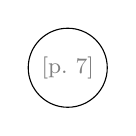
\begin{tikzpicture}
\node[draw,circle,inner sep=3pt] {\mspage{7}};
\end{tikzpicture}
\egroup
\typeout{LMWIDTH 95 \the\wd0 HEIGHT \the\ht0 DEPTH \the\dp0}
\typeout{LMSTART 96}
\setbox0=\hbox\bgroup
\begin{tikzcd}[ampersand replacement=\&,column sep=small,row sep=small]
\inserted{0=\unsure{\prod_i|\prod}\unsure{\Pi_2|\pi_2}(\operatorname{Aut}^+(C_i))}
\arrow[r] \&
\unsure{\Pi_1|\pi_1}(SA_{g,\nu}^{\prime0})\arrow[r] \&
\unsure{\Pi_1|\pi_1}(A_{g,\nu}^{\prime!+})\arrow[r]\arrow[d,equal] \&
\deleted{\unsure{\Pi_0}}\prod_i\unsure{\Pi_1|\pi_1}(\operatorname{Aut}^+(C_i))\arrow[r]\arrow[d,phantom,"\unsure{\wr}"] \&
\unsure{\Pi_0|\pi_0}(SA_{g,\nu}^{\prime+})\arrow[r] \&
\unsure{\Pi_0|\pi_0}(A_{g,\nu}^{\prime!+})\arrow[d,equal]\arrow[dd,bend left=28] \\
\&\&\unsure{\Pi_1|\pi_1}(A_{g,\nu}^{\prime0})\&\unsure{T^I}\&\overset{\uparrow}{\uline{\text{à calculer}}}\&\Gamma_{g,\nu}'\\
\&\&\&\&\&1=\prod_i\unsure{\Pi_0|\pi_0}(\operatorname{Aut}^+(C_i))
\end{tikzcd}
\egroup
\typeout{LMWIDTH 96 \the\wd0 HEIGHT \the\ht0 DEPTH \the\dp0}
\typeout{LMSTART 97}
\setbox0=\hbox\bgroup
\begin{tikzcd}[column sep=large,row sep=large,ampersand replacement=\&]
(24) \& 1 \arrow[r] \& \Pi_{g,\nu} \arrow[r] \arrow[dd] \& \unsure{\mathfrak{S}|\mathcal{G}}_{g,\nu}^{+} \arrow[r] \arrow[d,equal] \& \mathcal{T}_{g,\nu}^{+} \arrow[r] \arrow[d,equal] \& 1 \\
\& \& \& \pi_1(\unsure{U|\mathcal{U}}_{g,\nu\,C}) \arrow[d] \& \pi_1(M_{g,\nu\,C}) \arrow[d] \& \\
\text{(s'envoyant dans} \& 1 \arrow[r] \& \Pi_{g,\nu} \arrow[r] \& \operatorname{Aut}_{\mathrm{lac}}\deleted{\unsure{\mathrm{ext}}}(\Pi_{g,\nu}) \arrow[r] \arrow[d,equal] \& \operatorname{Aut\,ext}_{\mathrm{lac}}(\Pi_{g,\nu}) \arrow[r] \arrow[d,equal] \& 1 \\
\& \& \& \unsure{\mathfrak{S}|\mathcal{G}}_{g,\nu} \& \mathcal{T}_{g,\nu} \&
\end{tikzcd}
\egroup
\typeout{LMWIDTH 97 \the\wd0 HEIGHT \the\ht0 DEPTH \the\dp0}
\typeout{LMSTART 98}
\setbox0=\hbox\bgroup
\begin{tikzcd}[ampersand replacement=\&, column sep=small]
1 \arrow[r] \&
\pi_1(M_{g,\nu\overline{\mathbb Q}}) \arrow[r] \arrow[d, "{\unsure{\wr|2}}"] \&
\pi_1(M_{g,\nu}) \arrow[r, no head] \arrow[d] \&
\operatorname{Gal}(\overline{\mathbb Q}/\mathbb Q) \arrow[r] \arrow[d] \&
1 \\
1 \arrow[r] \&
\Sigma \arrow[r] \&
\unsure{\mathcal N|N}_\Sigma \arrow[r] \arrow[d, equal] \&
\Gamma_\Sigma \arrow[r] \arrow[dr] \&
1 \\
\& \&
\operatorname{Norm}_{\widehat{\widehat{\mathcal T}}(\pi)}(\Sigma) \&
\&
\text{\margin{groupe des autom. \deleted{\unsure{``arithmétiques}}\inserted{extérieurs} "arithmétiques" de $\pi$ (muni de $\Sigma$)}}
\end{tikzcd}
\egroup
\typeout{LMWIDTH 98 \the\wd0 HEIGHT \the\ht0 DEPTH \the\dp0}
\typeout{LMSTART 99}
\setbox0=\hbox\bgroup
\begin{tikzcd}[ampersand replacement=\&,column sep=large,row sep=large]
\& \&
\begin{gathered}
\text{Bases de }(\pi)\simeq\operatorname{Isom}_{\mathrm{lac}}(\widehat{\pi}_{g,\nu},\pi)\\
\downarrow\\
[\text{Bases}^{!}(\pi)\simeq\operatorname{Isom}^{!}_{\mathrm{lac}}(\widehat{\pi}_{g,\nu},\pi)]
\end{gathered}
\arrow[dl,"\mathcal G^{+}_{g,\nu}"']\arrow[dr,"\widehat{\pi}_{g,\nu}"]
\&\\
\&
\begin{gathered}
\text{discrétifications}\ \inserted{\text{orientées}}\ (\pi)\\
\simeq\operatorname{Isom}_{\mathrm{lac}}(\widehat{\pi}_{g,\nu},\pi)/\mathcal G^{+}_{g,\nu}\\
\simeq\operatorname{Isom}^{!}_{\mathrm{lac}}(\widehat{\pi}_{g,\nu},\pi)/\mathcal G^{!+}_{g,\nu}
\end{gathered}
\arrow[dl,"\{\pm1\}"']\arrow[dr]
\&\&
\begin{gathered}
\text{Bases extérieures de }\pi\\
\simeq\operatorname{Isom}\deleted{\,\mathrm{ext}}_{\mathrm{lac}}(\widehat{\pi}_{g,\nu},\pi)/\widehat{\pi}_{g,\nu}\\
\simeq\operatorname{Isom\,ext}_{\mathrm{lac}}(\widehat{\pi}_{g,\nu},\pi)\\
\downarrow\\
[\text{Bases ext}^{!}(\pi)\simeq\operatorname{Isom\,ext}^{!}_{\mathrm{lac}}(\widehat{\pi}_{g,\nu},\pi)]
\end{gathered}
\arrow[dl,"\mathcal T_{g,\nu}"]\\
\left[\begin{gathered}\text{Discrétifications }(\pi)\\\simeq\end{gathered}\right]
\arrow[d]
\&\&
\begin{gathered}
\text{prédiscrétifications}\ \inserted{\text{orientées}}\ \text{strictes}\ (\pi)\\
\simeq\operatorname{Isom}_{\mathrm{lac}}(\unsure{\widehat{\pi}}_{g,\nu},\pi)/\mathcal G^{+}_{g,\nu}\cdot\widehat{\pi}_{g,\nu}\\
\simeq\operatorname{Isom\,ext}_{\mathrm{lac}}(\widehat{\pi}_{g,\nu},\pi)/\mathcal T^{+}_{g,\nu})\\
\simeq\operatorname{Isom}^{!}(\widehat{\pi}_{g,\nu},\pi)/\mathcal G^{!+}_{g,\nu}\cdot\widehat{\pi}_{g,\nu}\\
\simeq\operatorname{Isom\,ext}_{\mathrm{lac}}(\widehat{\pi}_{g,\nu},\pi)/\mathcal T^{!+}_{g,\nu}
\end{gathered}
\arrow[dll,"\{\pm1\}"']\arrow[d]
\&\\
\left[\begin{gathered}\text{prédiscrétifications strictes}\\\text{de }\pi\\\simeq\end{gathered}\right]
\&\&
\begin{gathered}
\text{prédiscrétifications}\ \inserted{\text{orientées}}\ (\pi)\\
\simeq\operatorname{Isom}_{\mathrm{lac}}(\widehat{\pi}_{g,\nu},\pi)/\widehat{\mathcal G}^{+}_{g,\nu}\\
\simeq\operatorname{Isom\,ext}_{\mathrm{lac}}(\widehat{\pi}_{g,\nu},\pi)/\widehat{\mathcal T}^{+}_{g,\nu}\\
\deleted{\unsure{\simeq}}\quad
\simeq\operatorname{Isom}^{!}_{\mathrm{lac}}(\widehat{\pi}_{g,\nu},\pi)/\widehat{\mathcal G}^{!+}_{g,\nu}\\
\simeq\operatorname{Isom\,ext}^{!}_{\mathrm{lac}}(\widehat{\pi}_{g,\nu},\pi)/\widehat{\mathcal T}^{!+}_{g,\nu}
\end{gathered}
\arrow[dll,"\{\pm1\}"']\arrow[dd,"\Gamma_{\Sigma}"',"\Gamma_{g,\nu}"]
\&\\
\left[\begin{gathered}\text{prédiscrétifications de }\pi\\\simeq\end{gathered}\right]
\arrow[drr]
\&\&\&\\
\&\&
\begin{gathered}
\text{préarithmétisations de }\pi\\
\simeq\operatorname{Isom}_{\mathrm{lac}}(\widehat{\pi}_{g,\nu},\pi)/\mathcal M_{g,\nu}\\
\simeq\operatorname{Isom\,ext}_{\mathrm{lac}}(\widehat{\pi}_{g,\nu},\pi)/\mathcal N_{g,\nu}\\
\simeq\operatorname{Isom}^{!}_{\mathrm{lac}}(\widehat{\pi}_{g,\nu},\pi)/\mathcal M^{!}_{g,\nu}\\
\simeq\operatorname{Isom\,ext}^{!}_{\mathrm{lac}}(\widehat{\pi}_{g,\nu},\pi)/\mathcal N^{!}_{g,\nu}
\end{gathered}
\&
\end{tikzcd}
\egroup
\typeout{LMWIDTH 99 \the\wd0 HEIGHT \the\ht0 DEPTH \the\dp0}
\typeout{LMSTART 100}
\setbox0=\hbox\bgroup
\begin{tikzcd}[ampersand replacement=\&]
\deleted{\left\downarrow\vphantom{\rule{0pt}{2.8cm}}\right.}
\end{tikzcd}
\egroup
\typeout{LMWIDTH 100 \the\wd0 HEIGHT \the\ht0 DEPTH \the\dp0}
\typeout{LMSTART 101}
\setbox0=\hbox\bgroup
\begin{tikzcd}[ampersand replacement=\&,column sep=0.35cm,row sep=1.4cm,cells={nodes={inner sep=0pt,minimum size=0pt}}]
{} \& {} \arrow[d,bend right=8,line width=0.8pt,
  "{\widehat{\mathcal T}_{g,\nu}}"{pos=0.95,right}] \\
{} \& {} \arrow[dl,bend right=8,no head,line width=0.3pt] \\
{} \& {}
\end{tikzcd}
\egroup
\typeout{LMWIDTH 101 \the\wd0 HEIGHT \the\ht0 DEPTH \the\dp0}
\typeout{LMSTART 102}
\setbox0=\hbox\bgroup
\begin{tikzcd}[ampersand replacement=\&,column sep=0.30cm,row sep=0.40cm,cells={nodes={inner sep=0pt,minimum size=0pt}},arrows={line width=0.65pt,start anchor=center,end anchor=center,shorten <=1.2pt,shorten >=1.2pt}]
{} \& {} \& {} \arrow[dl] \arrow[dr] \& {} \& {} \arrow[ll] \arrow[dr] \& {} \\
|[yshift=-0.05cm]| {} \arrow[dr] \& {} \arrow[l] \arrow[dr] \& {} \& {} \arrow[dl] \& {} \& {} \arrow[ll] \\
{} \& |[yshift=-0.04cm]| {} \arrow[d] \& {} \arrow[l] \arrow[d] \& {} \& {} \& {} \\
{} \& |[yshift=-0.06cm]| {} \arrow[dr] \& {} \arrow[l] \arrow[dd,line width=1.25pt] \& {} \& {} \& {} \\
{} \& {} \& |[xshift=-0.12cm,yshift=-0.25cm]| {} \& {} \& {} \& {} \\
{} \& {} \& |[yshift=-0.45cm]| {} \& {} \& {} \& {}
\end{tikzcd}
\egroup
\typeout{LMWIDTH 102 \the\wd0 HEIGHT \the\ht0 DEPTH \the\dp0}
\typeout{LMSTART 103}
\setbox0=\hbox\bgroup
\begin{tikzcd}[ampersand replacement=\&,column sep=2.1em,row sep=3.0em]
1 \arrow[r,dash] \&
\pi_{g,\nu-1} \arrow[r,dash] \arrow[d,hook',no head] \&
\unsure{\mathcal T}_{g,\nu}^{!+} \arrow[r] \arrow[d,hook',no head] \&
\mathcal G_{g,\nu-1}^{!+} \arrow[r,dash] \arrow[d,hook',no head] \& 1 \\
1 \arrow[r,dash] \&
\widehat{\pi}_{g,\nu-1} \arrow[r] \arrow[d,equal] \&
\underset{\deleted{\unsure{\illegible{1}}}}{\widehat{\mathcal T}_{g,\nu}^{!+}}
\arrow[r] \arrow[d,hook',no head] \&
\widehat{\mathcal G}_{g,\nu-1}^{!+} \arrow[r,dash] \arrow[d,hook'] \& 1 \\
1 \arrow[r,dash] \&
\widehat{\pi}_{g,\nu-1} \arrow[r] \&
\widehat{\widehat{\mathcal T}}_{g,\nu}^{!} \arrow[r] \&
\widehat{\widehat{\mathcal G}}_{g,\nu-1}^{!} \arrow[r,dash] \& 1
\end{tikzcd}
\egroup
\typeout{LMWIDTH 103 \the\wd0 HEIGHT \the\ht0 DEPTH \the\dp0}
\typeout{LMSTART 104}
\setbox0=\hbox\bgroup
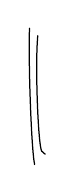
\begin{tikzpicture}[x=1cm,y=1cm,line width=.45pt,line cap=round]
\draw (0,0) .. controls (-.015,-.48) and (.025,-1.54) .. (.065,-1.73);
\draw (.105,-.095) .. controls (.070,-.48) and (.110,-1.48) .. (.155,-1.56) .. controls (.165,-1.58) and (.185,-1.59) .. (.200,-1.60);
\end{tikzpicture}
\egroup
\typeout{LMWIDTH 104 \the\wd0 HEIGHT \the\ht0 DEPTH \the\dp0}
\typeout{LMSTART 105}
\setbox0=\hbox\bgroup
\begin{tikzcd}[ampersand replacement=\&,column sep=large,row sep=huge]
\&
\deleted{\begin{gathered}
\Pi_1(\unsure{X(\mathbb C)}\setminus\{0,1,\infty\})\\[-2pt]
\rotatebox{90}{$=$}\\[-2pt]
\Pi_{0,3}
\end{gathered}}
\arrow[r,phantom,"{\deleted{\longleftarrow}}" description]
\&
\deleted{\begin{gathered}
\Pi_1\!\left(Y(\mathbb C)\setminus\{0,1,\infty\};
\underbrace{2\{1\}+3\{\infty\}}_{\substack{\text{signature de}\\\text{ramification}}}\right)\\[-2pt]
\rotatebox{90}{$=$}\\[-2pt]
\Pi'_{0,3}
\end{gathered}}
\\
(\deleted{\illegible{1}}\inserted{4}) \&
\left(\text{Rev. étales de }X\setminus\{0,1,\infty\}=U_{0,3}\right)
\arrow[r,phantom,"\simeq" description]
\arrow[d,phantom,"{\rotatebox{-90}{$\simeq$}}" description]
\&
\begin{gathered}
\left[\begin{gathered}
\text{Rev. de }Y\setminus\{0,1,\infty\}=U_{0,3}\\
\text{avec ramification sub. à}\\
\text{la signature }2\{1\}+3\{\infty\}
\end{gathered}\right]\\
\big/\begin{gathered}
\text{l'objet }(X\setminus\{0,1,\infty\})\\
\text{de la dite catégorie}
\end{gathered}
\end{gathered}
\arrow[d,phantom,"{\rotatebox{90}{$\simeq$}}" description]
\\
\& \Pi_{0,3}\text{-ensembles} \&
(\Pi'_{0,3}\text{-Ens})/\deleted{\unsure{E}}E
\end{tikzcd}
\egroup
\typeout{LMWIDTH 105 \the\wd0 HEIGHT \the\ht0 DEPTH \the\dp0}
\typeout{LMSTART 106}
\setbox0=\hbox\bgroup
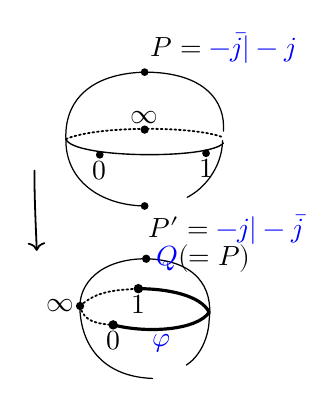
\begin{tikzpicture}[x=1cm,y=1cm,line cap=round,line join=round]
\draw[line width=.45pt] (0,2.85)
 .. controls (-.71,2.83) and (-1.02,2.47) .. (-1,2)
 .. controls (-1.01,1.48) and (-.57,1.16) .. (0,1.15);
\draw[line width=.45pt] (0,2.85)
 .. controls (.76,2.85) and (1.03,2.48) .. (1,2.10);
\draw[line width=.45pt] (.99,1.98)
 .. controls (.98,1.62) and (.74,1.36) .. (.54,1.26);
\draw[line width=.5pt] (-1,2)
 .. controls (-.91,1.75) and (.83,1.74) .. (1,1.95);
\draw[densely dotted,line width=.65pt] (-1,2)
 .. controls (-.61,2.17) and (.63,2.17) .. (1,2.02);
\fill (0,2.85) circle (1.4pt);
\node[anchor=south west,inner sep=2pt] at (0,2.88) {$P=\unsure{-\bar j|-j}$};
\fill (0,1.15) circle (1.4pt);
\node[anchor=north west,inner sep=2pt] at (-.03,1.12) {$P'=\unsure{-j|-\bar j}$};
\fill (-.57,1.80) circle (1.4pt);
\node[below,inner sep=2pt] at (-.57,1.80) {$0$};
\fill (.78,1.82) circle (1.4pt);
\node[below,inner sep=2pt] at (.78,1.82) {$1$};
\fill (0,2.12) circle (1.5pt);
\node[above,inner sep=2pt] at (0,2.12) {$\infty$};
\draw[->,line width=.65pt] (-1.40,1.60)
 .. controls (-1.40,1.22) and (-1.38,.85) .. (-1.37,.58);
\draw[line width=.45pt] (.02,.48)
 .. controls (-.55,.48) and (-.86,.17) .. (-.82,-.20)
 .. controls (-.78,-.70) and (-.46,-1.02) .. (.10,-1.04);
\draw[line width=.45pt] (.02,.48)
 .. controls (.65,.46) and (.87,.12) .. (.82,-.29)
 .. controls (.81,-.58) and (.66,-.79) .. (.53,-.87);
\fill (.02,.48) circle (1.5pt);
\node[anchor=west,inner sep=2pt] at (.07,.48) {$\unsure{Q}(=P)$};
\fill (-.82,-.12) circle (1.5pt);
\node[left,inner sep=2pt] at (-.82,-.12) {$\infty$};
\fill (-.08,.10) circle (1.7pt);
\node[below,inner sep=2pt] at (-.08,.10) {$1$};
\fill (-.40,-.36) circle (1.7pt);
\node[below,inner sep=2pt] at (-.40,-.36) {$0$};
\draw[line width=1.15pt] (-.08,.10)
 .. controls (.28,.10) and (.71,.02) .. (.82,-.20)
 .. controls (.66,-.43) and (.03,-.47) .. (-.40,-.36);
\draw[densely dotted,line width=.65pt] (-.82,-.12)
 .. controls (-.60,.08) and (-.36,.08) .. (-.08,.10);
\draw[densely dotted,line width=.65pt] (-.82,-.12)
 .. controls (-.78,-.32) and (-.59,-.35) .. (-.40,-.36);
\node[below,inner sep=1pt] at (.22,-.44) {$\unsure{\varphi}$};
\end{tikzpicture}
\egroup
\typeout{LMWIDTH 106 \the\wd0 HEIGHT \the\ht0 DEPTH \the\dp0}
\typeout{LMSTART 107}
\setbox0=\hbox\bgroup
\begin{tikzcd}[ampersand replacement=\&]
1 \arrow[r] \& \widehat{\Pi}_{03} \arrow[r] \arrow[d] \& \mathcal E_{03} \arrow[r] \arrow[d] \& \Gamma \arrow[r] \arrow[d,equal] \& 1 \\
1 \arrow[r] \& \widehat{\Pi}'_{03} \arrow[r] \& \mathcal E'_{03} \arrow[r] \& \Gamma \arrow[r] \& 1
\end{tikzcd}
\egroup
\typeout{LMWIDTH 107 \the\wd0 HEIGHT \the\ht0 DEPTH \the\dp0}
\typeout{LMSTART 108}
\setbox0=\hbox\bgroup
\begin{tikzcd}[ampersand replacement=\&,column sep=small]
\cdots \& E_2^{0,1} \arrow[r] \arrow[d,equal]
\& E_2^{2,0} \arrow[r] \arrow[d,equal]
\& \deleted{\unsure{E}}H^2(U_{0,3}) \arrow[r]
\& E_2^{1,1} \arrow[r] \arrow[d,equal]
\& E_2^{3,0} \arrow[d,equal] \& \cdots \\
\& H^0(\mathbb Q,H^1(\overline U)
\& H^2(\mathbb Q,\mathbb Z_{/2})
\&
\& H^1(\mathbb Q,\underset{\substack{\wr\\\mathbb F_2^2}}{H^1(\overline U)})
\& H^3(\mathbb Q,\unsure{\mathbb Z_{/2}|\mathbb F_2}) \&
\end{tikzcd}
\egroup
\typeout{LMWIDTH 108 \the\wd0 HEIGHT \the\ht0 DEPTH \the\dp0}
\typeout{LMSTART 109}
\setbox0=\hbox\bgroup
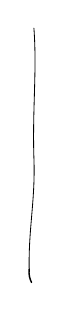
\begin{tikzpicture}[x=1cm,y=1cm,line cap=round]
\draw[line width=.30pt] (.04,0) .. controls (.08,-.55) and (.02,-1.02) .. (.04,-1.65)
 .. controls (.06,-2.18) and (-.03,-2.54) .. (-.02,-3.06);
\draw[line width=.52pt] (-.02,-3.06) .. controls (-.03,-3.13) and (-.01,-3.19) .. (.01,-3.23);
\end{tikzpicture}
\egroup
\typeout{LMWIDTH 109 \the\wd0 HEIGHT \the\ht0 DEPTH \the\dp0}
\typeout{LMSTART 110}
\setbox0=\hbox\bgroup
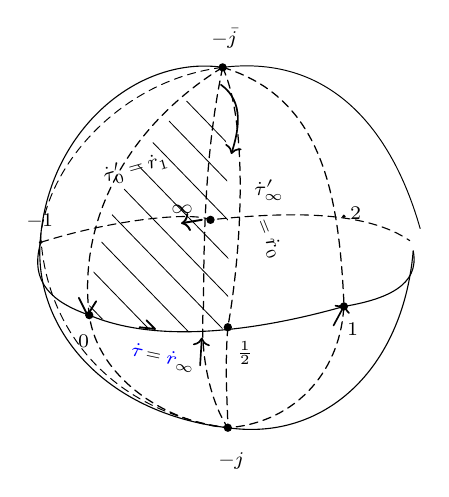
\begin{tikzpicture}[x=.022cm,y=-.022cm,line cap=round,line join=round,font=\scriptsize]
\coordinate (N) at (110,8);
\coordinate (S) at (113,216);
\draw[line width=.4pt] (N) .. controls (62,1) and (11,43) .. (5,105)
 .. controls (-1,158) and (42,208) .. (S)
 .. controls (168,224) and (214,183) .. (220,114);
\draw[line width=.35pt] (N) .. controls (175,0) and (209,48) .. (224,101);
\begin{scope}
\clip (N) .. controls (62,47) and (32,109) .. (33,151)
 .. controls (60,160) and (91,164) .. (113,158)
 .. controls (114,100) and (112,43) .. (N);
\foreach \a in {-80,-58,-36,-14,8,30,52,74,96,118,140,162}
  \draw[line width=.3pt] (-15,\a)--(145,{\a+165});
\end{scope}
\draw[dash pattern=on 3pt off 2pt,line width=.45pt] (N)
 .. controls (58,40) and (26,93) .. (33,151)
 .. controls (38,187) and (77,213) .. (S);
\draw[dash pattern=on 3pt off 2pt,line width=.45pt] (N)
 .. controls (101,51) and (99,95) .. (99,145)
 .. controls (96,180) and (106,206) .. (S);
\draw[dash pattern=on 3pt off 2pt,line width=.45pt] (N)
 .. controls (125,41) and (121,113) .. (113,158)
 .. controls (111,183) and (113,205) .. (S);
\draw[dash pattern=on 3pt off 2pt,line width=.45pt] (N)
 .. controls (167,25) and (177,80) .. (180,144)
 .. controls (179,182) and (153,213) .. (S);
\draw[dash pattern=on 3pt off 2pt,line width=.35pt] (N)
 .. controls (53,15) and (10,62) .. (5,105)
 .. controls (8,161) and (47,207) .. (S);
\draw[dash pattern=on 3pt off 2pt,line width=.4pt] (5,109)
 .. controls (46,96) and (92,91) .. (103,96)
 .. controls (150,91) and (193,91) .. (218,108);
\draw[line width=.4pt] (5,109) .. controls (-2,133) and (13,144) .. (33,151)
 .. controls (80,171) and (148,155) .. (180,146)
 .. controls (204,142) and (224,134) .. (220,114);
\draw[->,line width=.7pt] (98,96)--(86,98);
\draw[->,line width=.6pt] (109,18) .. controls (123,28) and (119,45) .. (115,58);
\draw[->,line width=.6pt] (97,180)--(98,164);
\draw[->,line width=.6pt] (174,157)--(181,144);
\draw[line width=.65pt] (27,141)--(32,151)--(37,143);
\draw[line width=.65pt] (62,158)--(71,159)--(66,154);
\foreach \p in {(110,8),(113,216),(103,96),(33,151),(113,158),(180,146)}
  \fill \p circle[radius=2.4];
\foreach \p in {(5,109),(180,94)}
  \fill \p circle[radius=1.1];
\node[inner sep=0pt] at (111,-9) {$-\bar j$};
\node[inner sep=0pt] at (115,235) {$-j$};
\node[inner sep=0pt] at (5,96) {$-1$};
\node[inner sep=0pt] at (87,90) {$\infty$};
\node[inner sep=0pt] at (187,92) {$2$};
\node[inner sep=0pt] at (30,166) {$0$};
\node[inner sep=0pt] at (123,173) {$\frac12$};
\node[inner sep=0pt] at (185,159) {$1$};
\node[inner sep=0pt,rotate=16] at (60,66) {$\dot\tau'_0=\dot r_1$};
\node[inner sep=0pt] at (137,79) {$\dot\tau'_\infty$};
\node[inner sep=0pt,rotate=-68] at (137,107) {$=\dot r_0$};
\node[inner sep=0pt,rotate=-12] at (76,176) {$\unsure{\dot\tau}=\unsure{\dot r}_\infty$};
\end{tikzpicture}
\egroup
\typeout{LMWIDTH 110 \the\wd0 HEIGHT \the\ht0 DEPTH \the\dp0}
\typeout{LMSTART 111}
\setbox0=\hbox\bgroup
\begin{tikzcd}[ampersand replacement=\&,column sep=large]
\widetilde{\uline{\varepsilon}}_0:\ G_a \arrow[r,hook] \& PG
\end{tikzcd}
\egroup
\typeout{LMWIDTH 111 \the\wd0 HEIGHT \the\ht0 DEPTH \the\dp0}
\typeout{LMSTART 112}
\setbox0=\hbox\bgroup
\begin{tikzcd}[ampersand replacement=\&,column sep=large]
\deleted{(\unsure{4})}\ (5)\quad\deleted{\unsure{\tau_{\rho,\sigma}}=}\ \mathrm{Gl}(2)
 \arrow[r,"\sim"] \& G
\end{tikzcd}
\egroup
\typeout{LMWIDTH 112 \the\wd0 HEIGHT \the\ht0 DEPTH \the\dp0}
\typeout{LMSTART 113}
\setbox0=\hbox\bgroup
\begin{tikzcd}[ampersand replacement=\&,column sep=large]
\mathcal R_{\rho,\sigma}^{\circ}
 \arrow[r,hook,"{\text{incl}}"'] \&
\mathcal M_{\rho,\sigma}^{\circ}
 \arrow[r,"{\text{can.}}"'] \&
\begin{gathered}
\mathcal T_{\rho,\sigma}^{\circ}\simeq T_\rho\mathbin{\times}_{\mathbb G_m}T_\sigma\\
\shortparallel\\[-3pt]
\mathcal M_{\rho,\sigma}^{\circ}/\widetilde{\mathcal G}_{\rho,\sigma}^{+}
\end{gathered}
\end{tikzcd}
\egroup
\typeout{LMWIDTH 113 \the\wd0 HEIGHT \the\ht0 DEPTH \the\dp0}
\typeout{LMSTART 114}
\setbox0=\hbox\bgroup
\begin{tikzcd}[ampersand replacement=\&,column sep=huge,row sep=large]
\mathcal R_{\rho,\sigma}^{\circ}
 \arrow[r,"{(73)}"]
 \arrow[d,"{\substack{\text{l'hom. can.}\\\text{de }(70)}}"']
 \arrow[dr,phantom,"{\text{cart}}",description] \&
T_\rho\mathbin{\times}_{\mathbb G_m}T_\sigma\simeq\mathcal T_{\rho,\sigma}^{\circ}
 \arrow[d,"{\text{can}}"]\\
\mathbb G_m \arrow[r,"{\mu\longmapsto\mu^2}"'] \&\mathbb G_m
\end{tikzcd}
\egroup
\typeout{LMWIDTH 114 \the\wd0 HEIGHT \the\ht0 DEPTH \the\dp0}
\typeout{LMSTART 115}
\setbox0=\hbox\bgroup
\begin{tikzcd}[ampersand replacement=\&,column sep=1.5em,row sep=5em]
\text{dim }3 \&
\begin{gathered}
\uline{\mathrm{Cent}}(\mathcal M_{\rho,\sigma}^{\circ})=R_{\rho,\sigma}^{\circ}\\
\simeq ST_\rho\times ST_\sigma\times G_m
\end{gathered}
\arrow[rr,hook,"{{{\substack{\text{(quotient}\\\mu_2\times\mu_2\text{)}}}}}"']
\& \&
\begin{gathered}
R_{\rho,\sigma}\\
\simeq S'T_\rho\times SN'_\sigma\times G_m
\end{gathered}
\&\text{dim }3\\
\text{dim }2\&
\begin{gathered}
\uline{\mathrm{Cent}}(\mathcal M_{\rho,\sigma})\cap\mathcal M_{\rho,\sigma}^{\circ}\\
=ST_\rho\times\mu_2\times G_m
\end{gathered}
\arrow[u,hook]\arrow[rr,hook,"{{{\substack{\text{(quotient}\\\mu_2\text{)}}}}}"']
\&\&
\begin{gathered}
\uline{\mathrm{Cent}}(\mathcal M_{\rho,\sigma})\\
\simeq S'T_\rho\times\deleted{\unsure{SN'_\sigma}}\inserted{\unsure{\mu_2}}\times G_m)
\end{gathered}
\arrow[u,hook]
\&\text{dim }2
\end{tikzcd}
\egroup
\typeout{LMWIDTH 115 \the\wd0 HEIGHT \the\ht0 DEPTH \the\dp0}
\typeout{LMSTART 116}
\setbox0=\hbox\bgroup
\begin{tikzcd}[ampersand replacement=\&,row sep=small,column sep=large]
 \& SG\arrow[dddr,"{j_G}"] \& \& G\arrow[r]\arrow[dr,"{\delta_G=\det_G}"] \& PG\\
 \& \& \& \& G_m\\
 \& S'T_\rho\arrow[dr,"{j_\rho}"] \& \& T_\rho\arrow[r,"{\delta_\rho=\det_{T_\rho}}"] \& G_m\\
\mu_2\arrow[uuur]\arrow[ur]\arrow[dr]\arrow[dddr]
 \& \& \mathcal{M}_{\rho,\sigma}\arrow[uuur,"{\Theta=\Theta_G}"]\arrow[ur,"{\Theta_\rho}"]\arrow[dr,"{\Theta_\sigma}"]\arrow[dddr,"{\varepsilon_3}"'] \& \& \\
 \& SN'_\sigma\arrow[ur,"{j_\sigma}"'] \& \& N'_\sigma\arrow[r,"{\delta'_\sigma=\det_{T_\sigma}}"]\arrow[dr,"{\varepsilon_\sigma}"] \& G_m\\
 \& \& \& \& \mu_2\\
 \& G_m\arrow[uuur,hook,"{j_\mu}"'] \& \& \mu_2 \&
\end{tikzcd}
\egroup
\typeout{LMWIDTH 116 \the\wd0 HEIGHT \the\ht0 DEPTH \the\dp0}
\typeout{LMSTART 117}
\setbox0=\hbox\bgroup
\begin{tikzcd}[ampersand replacement=\&,column sep=large]
G_m\arrow[r,"{i_\rho}"] \& T_\rho\arrow[r,"{\delta_\rho}"] \& G_m \& (\delta_\rho i_\rho(\lambda)=\lambda^2)
\end{tikzcd}
\egroup
\typeout{LMWIDTH 117 \the\wd0 HEIGHT \the\ht0 DEPTH \the\dp0}
\typeout{LMSTART 118}
\setbox0=\hbox\bgroup
\begin{tikzcd}[ampersand replacement=\&,column sep=large]
G_m\arrow[r,"{i_\sigma}"] \& N'_\sigma\arrow[r,"{\delta_\sigma}"] \& G_m \& (\delta_\sigma i_\sigma(\lambda)=\lambda^2)
\end{tikzcd}
\egroup
\typeout{LMWIDTH 118 \the\wd0 HEIGHT \the\ht0 DEPTH \the\dp0}
\typeout{LMSTART 119}
\setbox0=\hbox\bgroup
\begin{tikzcd}[ampersand replacement=\&,column sep=large]
 \& N'_\sigma\arrow[r,"{\varepsilon_\sigma}"] \& \mu_2 \& \varepsilon_\sigma i_\sigma(\lambda)=1
\end{tikzcd}
\egroup
\typeout{LMWIDTH 119 \the\wd0 HEIGHT \the\ht0 DEPTH \the\dp0}
\typeout{LMSTART 120}
\setbox0=\hbox\bgroup
\begin{tikzcd}[ampersand replacement=\&,column sep=large]
1\arrow[r] \& G_m\arrow[r]\arrow[dr,phantom,"{\text{cart}}" description] \& G\arrow[r] \& PG\arrow[r] \& 1\\
1\arrow[r] \& \mu_2\arrow[u,hook]\arrow[r] \& SG\arrow[u,hook]\arrow[r] \& PG\arrow[u,equal]\arrow[r] \& 1
\end{tikzcd}
\egroup
\typeout{LMWIDTH 120 \the\wd0 HEIGHT \the\ht0 DEPTH \the\dp0}
\typeout{LMSTART 121}
\setbox0=\hbox\bgroup
\begin{tikzcd}[ampersand replacement=\&,column sep=large,row sep=large]
 \& 1 \& 1 \& \&\\
 \& G_m\arrow[u]\arrow[r,equal] \& G_m\arrow[u] \& \&\\
1\arrow[r] \& G_m\arrow[u,"{\lambda\mapsto\lambda^2}"]\arrow[r,hook,"{\unsure{j}}"] \& G\arrow[u,"{\delta_G}"]\arrow[r] \& PG\arrow[r] \& 1\\
1\arrow[r] \& \mu_2\arrow[u,hook]\arrow[r] \& SG\arrow[u,hook]\arrow[r] \& PG\arrow[u,equal]\arrow[r] \& 1\\
 \& 1\arrow[u] \& \unsure{0|1}\arrow[u] \& \&
\end{tikzcd}
\egroup
\typeout{LMWIDTH 121 \the\wd0 HEIGHT \the\ht0 DEPTH \the\dp0}
\typeout{LMSTART 122}
\setbox0=\hbox\bgroup
\begin{tikzcd}[ampersand replacement=\&,column sep=large]
\mathcal T_{1,1}^{\unsure{*|+}\wedge}\simeq\mathrm{GL}(2,\mathbb Z)^{\wedge}
\arrow[r,"\text{épi}"] \& \mathcal G
\end{tikzcd}
\egroup
\typeout{LMWIDTH 122 \the\wd0 HEIGHT \the\ht0 DEPTH \the\dp0}
\typeout{LMSTART 123}
\setbox0=\hbox\bgroup
\begin{tikzcd}
1\arrow[r]&\unsure{Z_\rho|L_\rho}\arrow[r]&N_\rho\arrow[r,"\varepsilon_\rho"]&\{\pm1\}\arrow[r]&1\\
1\arrow[r]&Z_\sigma\arrow[r]&N_\sigma\arrow[r,"\varepsilon_\sigma"]&\{\pm1\}\arrow[r]&1
\end{tikzcd}
\egroup
\typeout{LMWIDTH 123 \the\wd0 HEIGHT \the\ht0 DEPTH \the\dp0}
\typeout{LMSTART 124}
\setbox0=\hbox\bgroup
\begin{tikzcd}[row sep=small,column sep=large]
&\mathbb D_\rho\arrow[r]&N_\rho\arrow[dr,"i_\rho"]&\\
\{1,\tau'\}\times\{\pm1\}\arrow[ur,hook]\arrow[dr,hook]&&&G_{\rho,\sigma}\\
&\mathbb D_\sigma\arrow[r]&N_\sigma\arrow[ur,"\unsure{i_\sigma}"']&
\end{tikzcd}
\egroup
\typeout{LMWIDTH 124 \the\wd0 HEIGHT \the\ht0 DEPTH \the\dp0}
\typeout{LMSTART 125}
\setbox0=\hbox\bgroup
\begin{tikzcd}
\mathbb D_\rho\arrow[r]&N_\rho,
\end{tikzcd}
\egroup
\typeout{LMWIDTH 125 \the\wd0 HEIGHT \the\ht0 DEPTH \the\dp0}
\typeout{LMSTART 126}
\setbox0=\hbox\bgroup
\begin{tikzcd}
\mathbb D_\sigma\arrow[r]&N_\sigma
\end{tikzcd}
\egroup
\typeout{LMWIDTH 126 \the\wd0 HEIGHT \the\ht0 DEPTH \the\dp0}
\typeout{LMSTART 127}
\setbox0=\hbox\bgroup
\begin{tikzcd}[column sep=large,row sep=small]
&L_0\simeq SZ_{\rho,\sigma}\arrow[rr]\arrow[ddd,hook]&&Z_{\rho,\sigma}
\arrow[ddd,hook,dashed]\arrow[dddrr,dashed,"\delta_Z"]&&&\\
&&SN_\rho^*\arrow[rr]\arrow[ddl,hook]& &N_\rho^*
\arrow[ddl,hook,dashed]\arrow[ddr,dashed,"\delta_\rho"]&&
\widehat{\mathbb Z}^{*}\times\{\pm1\}\times\{\pm1\}\\
&&SN_\sigma^*\arrow[rr]\arrow[dl,hook,dotted]\arrow[dl]&&N_\sigma^*
\arrow[dl,hook,dotted]\arrow[dl]\arrow[dr,dashed,"\delta_\sigma"]&&\\
1\arrow[r]&\mathcal G^+\arrow[rr,hook,"i_{\mathcal G^+}"]\arrow[dr,hook]&&
G_{\rho,\sigma}\arrow[rr,"\delta_G"]&&\gamma_{\rho,\sigma}\arrow[r]\arrow[uur,"{(\chi_\gamma,\varepsilon_{\gamma,\rho},\varepsilon_{\gamma,\sigma})}"]&1\\
&&\mathcal G\arrow[ur,hook]&&&&
\end{tikzcd}
\egroup
\typeout{LMWIDTH 127 \the\wd0 HEIGHT \the\ht0 DEPTH \the\dp0}
\typeout{LMSTART 128}
\setbox0=\hbox\bgroup
\begin{tikzcd}[column sep=small,row sep=large]
 & & L_0\times SN_\rho^*\times SN_\sigma^*
 & & & & L_0 & & & &\\
 & & & & S_0\Gamma_{\rho,\sigma}
 & & & & Z_{\rho,\sigma} & &\\
L_0\times SN_\rho^*\times SN_\sigma^*\times\mathcal G^+
 & & SN_\rho^*\times SN_\sigma^*
 & & & & \mathrm{III}^{\unsure{+|'}}
 & & & &\\
 & & & S_0\mathcal M_{\rho,\sigma}
 & \Gamma_{\rho,\sigma} & & N_\rho^*
 & & & & \{\pm1\}\\
 & SN_\rho^*\times SN_\sigma^*\times\mathcal G^+
 & & & & & N_\sigma^*
 & & \gamma_{\rho,\sigma} & & \widehat{\mathbb Z}^{*}\\
 & & & & & \mathrm{II}
 & \deleted{\unsure{\mathcal G^+|N_\sigma^*}}
 & & & & \{\pm1\}\\
 & & & \mathcal M_{\rho,\sigma}
 & & & & & G_{\rho,\sigma} & &\\
\mathcal G^+ & & & & & & & & & &\\
 & & \mathcal G & & & & & & & &\\
 & & \Vert & & & & & & & &\\
 & & \{1,\tau'\}\mathbin{.}\mathcal G^+
 & & & & & & & &
\arrow[from=1-3,to=1-7,"\mathrm{pr}"]
\arrow[from=1-3,to=2-5,hook]
\arrow[from=1-3,to=3-3,"\mathrm{pr}"]
\arrow[from=1-7,to=2-9,hook]
\arrow[from=2-5,to=2-9,"\theta_Z"]
\arrow[from=2-5,to=4-5]
\arrow[from=2-9,to=5-9,"\delta_Z"]
\arrow[from=3-1,to=1-3,"\mathrm{pr}"]
\arrow[from=3-1,to=5-2,"\mathrm{pr}"']
\arrow[from=3-1,to=4-4,hook]
\arrow[from=3-3,to=4-5,hook]
\arrow[from=4-4,to=2-5]
\arrow[from=4-4,to=7-4]
\arrow[from=4-5,to=4-7,"\theta_\rho"]
\arrow[from=4-5,to=5-7,"\theta_\sigma"']
\arrow[from=4-7,to=5-9,"\delta_\rho"]
\arrow[from=5-7,to=5-9,"\delta_\sigma"]
\arrow[from=5-2,to=3-3,"\mathrm{pr}"']
\arrow[from=5-2,to=7-4,hook]
\arrow[from=5-2,to=6-7,dashed,"\unsure{\mathrm{pr}}"]
\arrow[from=6-7,to=7-9,dashed,hook]
\arrow[from=7-4,to=4-5]
\arrow[from=7-4,to=6-7,dotted]
\arrow[from=7-4,to=7-9,"\theta_G"]
\arrow[from=7-9,to=5-9,"\delta_G"']
\arrow[from=5-9,to=4-11,
 "{\varepsilon_{\gamma,\rho}=\varepsilon'_\gamma}"]
\arrow[from=5-9,to=5-11,"\chi_\gamma"]
\arrow[from=5-9,to=6-11,
 "{\varepsilon_{\gamma,\sigma}=\varepsilon_\gamma}"']
\arrow[from=8-1,to=5-2,hook,"\uline{\mathrm{inj}}"]
\arrow[from=8-1,to=7-4,dashed]
\arrow[from=8-1,to=9-3,hook]
\arrow[from=9-3,to=7-4,hook,"i_{\mathcal G,\mathcal M}"]
\arrow[from=9-3,to=7-9,dashed,hook,"i_{\mathcal G,G}"']
\arrow[from=1-3,to=2-9,phantom,
 "{\deleted{\unsure{\mathrm{IV}}}\ \mathrm{V}}" description,pos=.52]
\arrow[from=4-7,to=5-7,phantom,"\mathrm{I}" description]
\arrow[from=8-1,to=7-4,phantom,"\mathrm{IV}" description,pos=.5]
\end{tikzcd}
\egroup
\typeout{LMWIDTH 128 \the\wd0 HEIGHT \the\ht0 DEPTH \the\dp0}
\typeout{LMSTART 129}
\setbox0=\hbox\bgroup
\begin{tikzcd}
\mathcal G^+\arrow[r] &
SN_\rho^*\times SN_\sigma^*\times\mathcal G^+
\end{tikzcd}
\egroup
\typeout{LMWIDTH 129 \the\wd0 HEIGHT \the\ht0 DEPTH \the\dp0}
\typeout{LMSTART 130}
\setbox0=\hbox\bgroup
\begin{tikzcd}
Z_{\rho,\sigma}\arrow[r] & G_{\rho,\sigma},
\end{tikzcd}
\egroup
\typeout{LMWIDTH 130 \the\wd0 HEIGHT \the\ht0 DEPTH \the\dp0}
\typeout{LMSTART 131}
\setbox0=\hbox\bgroup
\begin{tikzcd}
N_\rho^*\arrow[r] & G_{\rho,\sigma},
\end{tikzcd}
\egroup
\typeout{LMWIDTH 131 \the\wd0 HEIGHT \the\ht0 DEPTH \the\dp0}
\typeout{LMSTART 132}
\setbox0=\hbox\bgroup
\begin{tikzcd}
N_\sigma^*\arrow[r] & G_{\rho,\sigma}
\end{tikzcd}
\egroup
\typeout{LMWIDTH 132 \the\wd0 HEIGHT \the\ht0 DEPTH \the\dp0}
\typeout{LMSTART 133}
\setbox0=\hbox\bgroup
\begin{tikzcd}[column sep=large,row sep=large]
\mu\simeq\{1,\tau_{\mathcal E}\}\arrow[r]&\mu\times\mu&
\tau_{\mathcal E}\arrow[r,mapsto]&(-1,-1)\quad\text{(hom diagonal)}\\
\mathcal E''\arrow[r]&\unsure{\mu\times\{1\}}\arrow[r,hook]&\mu\times\mu&
\end{tikzcd}
\egroup
\typeout{LMWIDTH 133 \the\wd0 HEIGHT \the\ht0 DEPTH \the\dp0}
\typeout{LMSTART 134}
\setbox0=\hbox\bgroup
\begin{tikzcd}
\mathcal E''_2\overset{\mathrm{dfn}}{=}
\unsure{\mathcal E''/2\mathcal E''|\mathcal E''/{}_{2}\mathcal E''}
\arrow[r,"\sim"]&\mu
\end{tikzcd}
\egroup
\typeout{LMWIDTH 134 \the\wd0 HEIGHT \the\ht0 DEPTH \the\dp0}
\typeout{LMSTART 135}
\setbox0=\hbox\bgroup
\begin{tikzcd}
 \gamma_{\rho,\sigma}\arrow[r]\arrow[d,phantom,"\Vert"] & N^*_{\rho}/\{\pm1\}\\
 \Gamma_{\mathbb Q}^{\sim}
\end{tikzcd}
\egroup
\typeout{LMWIDTH 135 \the\wd0 HEIGHT \the\ht0 DEPTH \the\dp0}
\typeout{LMSTART 136}
\setbox0=\hbox\bgroup
\begin{tikzcd}[column sep=large,row sep=huge]
 \mathcal M^![0]=Z^!_{\rho,\sigma}\arrow[rr,"\text{can}"]
 &&\gamma_{\rho,\sigma}=Z^!_{\rho,\sigma}/L_0^{\Pi}
       \arrow[r,"\text{hom }(130)"]
 &N^*_{\rho}/\{\pm1\}\\
 S_0\Gamma^!_{\rho,\sigma}
       \arrow[u,"{\text{can}\quad(u,a,b)\mapsto u}"']
 &\inserted{\unsure{S_0}\Gamma_{\rho,\sigma}\quad\text{(sans !)}}
       \arrow[ur,very thick,"{\substack{\text{can}\\\unsure{\text{(passage au quotient)}}}}"']
 &&\\
 S_0^{\Pi}\Gamma^!_{\rho,\sigma}\arrow[u,hook,"\text{incl.}"']
       \arrow[ur,hook,dashed,"\text{incl.}"']\arrow[rrr]
 &&&N^*_{\rho}\arrow[uu]
\end{tikzcd}
\egroup
\typeout{LMWIDTH 136 \the\wd0 HEIGHT \the\ht0 DEPTH \the\dp0}
\typeout{LMSTART 137}
\setbox0=\hbox\bgroup
\begin{tikzcd}[column sep=large,row sep=huge]
 \mathcal M(0)\arrow[r,hook]\arrow[dr,phantom,"\mathrm I" description]
 &\mathcal M^![0]=Z^!_{\rho,\sigma}\arrow[r,"\text{épi}"]
       \arrow[dr,phantom,"\mathrm {II}" description]
 &\gamma_{\rho,\sigma}\arrow[r,hook]
       \arrow[dr,phantom,"\mathrm {III}" description]
 &N^*_{\rho}/\{\pm1\}\\
 \mathcal M(0)^{\sim}\arrow[u]\arrow[r,hook]
 &S_0^{\Pi}\Gamma^!_{\rho,\sigma}\arrow[u,"2"]\arrow[r]
 &\widetilde\gamma_{\rho,\sigma}\arrow[u,"2"]\arrow[r,hook]
 &N_{\rho}^{\unsure{*|d}}\arrow[u,"2"]
\end{tikzcd}
\egroup
\typeout{LMWIDTH 137 \the\wd0 HEIGHT \the\ht0 DEPTH \the\dp0}
\typeout{LMSTART 138}
\setbox0=\hbox\bgroup
\begin{tikzcd}[column sep=small,row sep=small]
1 \arrow[r] & \mu \arrow[r] & Z_\rho^{*!} \arrow[r] & \gamma_{\rho,\sigma} \arrow[r] \arrow[d,phantom,"\rotatebox{90}{$\simeq$}"] & 1 \\
& & (\simeq\widetilde{\gamma}_{\rho,\sigma}) & \widetilde{\Gamma}_{\mathbb Q} &
\end{tikzcd}
\egroup
\typeout{LMWIDTH 138 \the\wd0 HEIGHT \the\ht0 DEPTH \the\dp0}
\typeout{LMSTART 139}
\setbox0=\hbox\bgroup
\begin{tikzcd}
\gamma_{\rho,\sigma}\simeq Z_\rho^{*!}/\mu \arrow[r] & N_\rho^*/\mu
\end{tikzcd}
\egroup
\typeout{LMWIDTH 139 \the\wd0 HEIGHT \the\ht0 DEPTH \the\dp0}
\typeout{LMSTART 140}
\setbox0=\hbox\bgroup
\begin{tikzcd}[ampersand replacement=\&,column sep=1.05em,row sep=2.8em]
\&\& \mathcal{M}^{0}(-\bar j)
  \arrow[rr,hook,"2"]
  \arrow[dl,hook,"2"']
\&\& \begin{gathered}\mathcal{M}'(-\bar j)\\=Z_{\rho,0}^{!}\end{gathered}
  \arrow[rr,hook,"2"]
  \arrow[dl,hook,"2"']
  \arrow[dr,no head,draw=gray,
    "{\unsure{\mathcal{M}'(-\bar j)\times\mu}}"{description,pos=.5},
    "{\unsure{\searrow}}"{pos=.93}]
\&\& \mathcal{M}'(-\bar j)\times\mu
  \arrow[rr,hook,"3"]
  \arrow[dl,hook,"2"']
\&\& Z_{\rho}\arrow[dl,hook,"2"']\\
(37)\&\mathcal{M}'''(-\bar j)\arrow[rr,hook,"2"]
\&\& \mathcal{M}'''(-\bar j)\times\mu\arrow[rr,hook,"2"]
\&\& \mathcal{N}_{\rho}^{?}\arrow[rr,hook,"3"]
\&\& \mathcal{N}_{\rho}^{*}
\&\&\\
\&\&\&\&1
  \arrow[uu,hook]
  \arrow[uull,hook,start anchor=north west,end anchor=south west]
  \arrow[rr,hook,"2"]
  \arrow[dl,hook,"2"']
\&\&\mu\arrow[uu,hook]\arrow[rr,hook,"3"]\arrow[dl,hook,"2"']
\&\&L_{\rho}\arrow[uu,hook]\arrow[dl,hook,"2"']\\
\&\&\&\mu_{\tau'}\arrow[uu,hook]\arrow[uull,hook]\arrow[rr,hook,"2"]
\&\&\mathbb{D}_{\tau'}\arrow[uu,hook]\arrow[rr,hook,"3"]
\&\&\mathbb{D}_{\rho}\arrow[uu,hook]
\end{tikzcd}
\egroup
\typeout{LMWIDTH 140 \the\wd0 HEIGHT \the\ht0 DEPTH \the\dp0}
\typeout{LMSTART 141}
\setbox0=\hbox\bgroup
\begin{tikzcd}[ampersand replacement=\&, column sep=large]
Z_{\rho,\sigma}\arrow[r,hook]\&\operatorname{Aut}(\mathcal{G}^{+})
\end{tikzcd}
\egroup
\typeout{LMWIDTH 141 \the\wd0 HEIGHT \the\ht0 DEPTH \the\dp0}
\typeout{LMSTART 142}
\setbox0=\hbox\bgroup
\begin{tikzcd}[ampersand replacement=\&, column sep=large,row sep=large]
M[0]\arrow[r,"\sim"]\arrow[d,equal]\&
\widetilde{M}_{0,3}[0]\arrow[d,equal]\\
M(\unsure{\omega|0}).L_0^{\mathcal{G}}\arrow[r,"\sim"]\&
\unsure{M_{0,3}(0)}.
L_0^{\tikz[baseline=(g.base)]{\node[draw,ellipse,inner sep=1pt]
(g){$\scriptstyle\unsure{\mathcal{G}_{0,3}}$};}}
\end{tikzcd}
\egroup
\typeout{LMWIDTH 142 \the\wd0 HEIGHT \the\ht0 DEPTH \the\dp0}
\typeout{LMSTART 143}
\setbox0=\hbox\bgroup
\begin{tikzcd}[ampersand replacement=\&]
(19)\quad L_0^{\unsure{\natural|\sharp}}
  \arrow[r,"\unsure{i}"] \& Z_{\rho,\sigma},\\
l \arrow[r,mapsto] \& (\operatorname{int}_{\mathcal{G}^{+}}(l),1,1,1)
\end{tikzcd}
\egroup
\typeout{LMWIDTH 143 \the\wd0 HEIGHT \the\ht0 DEPTH \the\dp0}
\typeout{LMSTART 144}
\setbox0=\hbox\bgroup
\begin{tikzcd}[ampersand replacement=\&]
(22)\quad 1 \arrow[r] \&
L_0^{\unsure{\natural|\sharp}} \arrow[r] \&
Z_{\rho,\sigma} \arrow[r,"\delta_Z"] \&
\gamma_{\rho,\sigma} \arrow[r] \& 1,
\end{tikzcd}
\egroup
\typeout{LMWIDTH 144 \the\wd0 HEIGHT \the\ht0 DEPTH \the\dp0}
\typeout{LMSTART 145}
\setbox0=\hbox\bgroup
\begin{tikzcd}[ampersand replacement=\&]
 \& \& \mu\\
(23)\quad Z_{\rho,\sigma} \arrow[r] \&
\gamma_{\rho,\sigma}
  \arrow[ur,"\varepsilon_{3\gamma}"]
  \arrow[r,"\chi_\gamma"]
  \arrow[dr,"\varepsilon_{2\gamma}"'] \&
\widehat{\mathbb{Z}}^{*}\\
 \& \& \mu
\end{tikzcd}
\egroup
\typeout{LMWIDTH 145 \the\wd0 HEIGHT \the\ht0 DEPTH \the\dp0}
\typeout{LMSTART 146}
\setbox0=\hbox\bgroup
\begin{tikzcd}[ampersand replacement=\&, row sep=0pt]
 \& \varepsilon_3\\
(u,\mu,\varepsilon_2,\varepsilon_3)
  \arrow[ur,mapsto] \arrow[r,mapsto] \arrow[dr,mapsto]
  \& \mu\\
 \& \varepsilon_2.
\end{tikzcd}
\egroup
\typeout{LMWIDTH 146 \the\wd0 HEIGHT \the\ht0 DEPTH \the\dp0}
\typeout{LMSTART 147}
\setbox0=\hbox\bgroup
\begin{tikzcd}[ampersand replacement=\&]
Z_{\rho,\sigma}\arrow[r]\&\operatorname{Aut}(\mathcal{G}^{+})
\end{tikzcd}
\egroup
\typeout{LMWIDTH 147 \the\wd0 HEIGHT \the\ht0 DEPTH \the\dp0}
\typeout{LMSTART 148}
\setbox0=\hbox\bgroup
\begin{tikzcd}[ampersand replacement=\&]
(28)\quad L_0^{\unsure{\natural|\sharp}}
  \arrow[r,hook,"\unsure{i_{L_0,S_0G}|i_{L_0,G}}"]\&
S_0G_{\rho,\sigma}^{\unsure{\natural|\sharp}}
  \arrow[r,phantom,"\subset"]\&S_0G_{\rho,\sigma}\\
l\arrow[r,mapsto]\&
\deleted{\unsure{\iota(l)|i(l)}}\,i_{L_0,Z}(l)\mathbin{.}l^{-1}
\end{tikzcd}
\egroup
\typeout{LMWIDTH 148 \the\wd0 HEIGHT \the\ht0 DEPTH \the\dp0}
\typeout{LMSTART 149}
\setbox0=\hbox\bgroup
\begin{tikzcd}[ampersand replacement=\&, column sep=small,row sep=large]
Z_0^{\unsure{\natural|\sharp}}\arrow[rr]\&\&
S_0G_{\rho,\sigma}^{\unsure{\natural|\sharp}}
=Z_{\rho,\sigma}\cdot\mathcal G^{\unsure{\natural|\sharp}}
\&\&\\
f\arrow[r,mapsto]\&
f^{-1}\arrow[d,phantom,"\in"{rotate=-90}]\&
{\cdot\uline{u}(f)}\arrow[d,phantom,"\in"{rotate=-90}]\&
\inserted{=\uline{u}(f)\cdot f^{-1}}\&
{\text{où }\uline{u}(f)=(\operatorname{int}(f),1,1,1)
\in Z_{\rho,\sigma}}\arrow[d,phantom,"\subset"{rotate=-90}]\\
\&\mathcal G^{\unsure{\natural|\sharp}}\&
Z_{\rho,\sigma}\&\&G_{\rho,\sigma}^{\unsure{\natural|\sharp}}
\end{tikzcd}
\egroup
\typeout{LMWIDTH 149 \the\wd0 HEIGHT \the\ht0 DEPTH \the\dp0}
\typeout{LMSTART 150}
\setbox0=\hbox\bgroup
\begin{tikzcd}[ampersand replacement=\&]
Z_0^{\unsure{\natural|\sharp}}/L_0^{\unsure{\natural|\sharp}}
\arrow[r,hook]\&G_{\rho,\sigma}^{\unsure{\natural|\sharp}}
\end{tikzcd}
\egroup
\typeout{LMWIDTH 150 \the\wd0 HEIGHT \the\ht0 DEPTH \the\dp0}
\typeout{LMSTART 151}
\setbox0=\hbox\bgroup
\begin{tikzcd}[ampersand replacement=\&, column sep=small,row sep=large]
1\arrow[r]\&
L_0^{\unsure{\natural|\sharp}}\arrow[r]\&
Z_0^{\unsure{\natural|\sharp}}\arrow[r]\&
G_{\rho,\sigma}^{\unsure{\natural|\sharp}}\arrow[r]\&
\widetilde G_{\rho,\sigma}^{\unsure{\natural|\sharp}}
\arrow[r]\arrow[d,phantom,"\subset"{rotate=-90}]\&1\\
\&\&\&\&
{\operatorname{Aut}(\mathcal G^+)\times\widehat{\mathbb Z}^{*}\times\mu\times\mu}
\&
\end{tikzcd}
\egroup
\typeout{LMWIDTH 151 \the\wd0 HEIGHT \the\ht0 DEPTH \the\dp0}
\typeout{LMSTART 152}
\setbox0=\hbox\bgroup
\begin{tikzcd}[column sep=large]
\text{(35)} &
\begin{gathered}
\underline{\mathcal G}\supset\underline M\\[-2pt]
\text{Groupe sur }S_0,\\[-2pt]
\text{avec }\underline M\text{ comme}\\[-2pt]
\text{sous-groupe distingué}
\end{gathered}
& \text{, et }\Phi\colon\mathcal G_{S_0}\arrow[r]
& \underline{\mathcal G}
\end{tikzcd}
\egroup
\typeout{LMWIDTH 152 \the\wd0 HEIGHT \the\ht0 DEPTH \the\dp0}
\typeout{LMSTART 153}
\setbox0=\hbox\bgroup
\begin{tikzcd}
\underbrace{\mathcal G_{S_0}/M_{S_0}}_{H_{S_0}}
\arrow[r,"\sim"] & \underline{\mathcal G}/\underline M
\end{tikzcd}
\egroup
\typeout{LMWIDTH 153 \the\wd0 HEIGHT \the\ht0 DEPTH \the\dp0}
\typeout{LMSTART 154}
\setbox0=\hbox\bgroup
\begin{tikzcd}[column sep=large,row sep=small]
\text{(36)} & 1\arrow[r,dash] & \underline M\arrow[r]
& \underline{\mathcal G}\arrow[r]
& \underline{\mathcal G}/\underline M\arrow[r,dash]
\arrow[d,phantom,"\simeq"{description,rotate=90}] & 1\\
&&&& H_{S_0}.
\end{tikzcd}
\egroup
\typeout{LMWIDTH 154 \the\wd0 HEIGHT \the\ht0 DEPTH \the\dp0}
\typeout{LMSTART 155}
\setbox0=\hbox\bgroup
\begin{tikzcd}[column sep=large,row sep=small]
\text{(37)} & 1\arrow[r] & \underline M(S)\arrow[r]
\arrow[d,phantom,"\simeq"{description,rotate=90}]
& \underline{\mathcal G}\unsure{(A)|(/A)}\arrow[r]
& H_{S_0}(S)\arrow[r,dash]
\arrow[d,phantom,"\simeq"{description,rotate=90}] & 1\\
&& M\otimes_{\mathbb Z}A && H\text{ si }S\text{ conn.}\\[-3pt]
&&\text{si }S\text{ affine d'anneau }A
\end{tikzcd}
\egroup
\typeout{LMWIDTH 155 \the\wd0 HEIGHT \the\ht0 DEPTH \the\dp0}
\typeout{LMSTART 156}
\setbox0=\hbox\bgroup
\begin{tikzcd}[column sep=large]
\underline M_{S_0}\arrow[r,"u_{\underline M}"] & \unsure{G^{\sharp}|G^{\natural}}
\end{tikzcd}
\egroup
\typeout{LMWIDTH 156 \the\wd0 HEIGHT \the\ht0 DEPTH \the\dp0}
\typeout{LMSTART 157}
\setbox0=\hbox\bgroup
\begin{tikzcd}[column sep=large]
\unsure{C_{S_0}|G_{S_0}}\arrow[r,"u_{\unsure{C|G}}"] & \unsure{G^{\sharp}|G^{\natural}}
\end{tikzcd}
\egroup
\typeout{LMWIDTH 157 \the\wd0 HEIGHT \the\ht0 DEPTH \the\dp0}
\typeout{LMSTART 158}
\setbox0=\hbox\bgroup
\begin{tikzcd}[column sep=large]
\unsure{C|G}\arrow[r] & \unsure{G^{\sharp}(S_0)|G^{\natural}(S_0)}
\end{tikzcd}
\egroup
\typeout{LMWIDTH 158 \the\wd0 HEIGHT \the\ht0 DEPTH \the\dp0}
\typeout{LMSTART 159}
\setbox0=\hbox\bgroup
\begin{tikzcd}[column sep=large,row sep=large]
M_{S_0}\arrow[r]\arrow[d] & \unsure{C^+_{S_0}|G^+_{S_0}}\arrow[ddr,"u_{\unsure{C|G}}"] & \\
\underline M_{S_0}\arrow[drr,"u_{\underline M}"'] & & \\
& & G
\end{tikzcd}
\egroup
\typeout{LMWIDTH 159 \the\wd0 HEIGHT \the\ht0 DEPTH \the\dp0}
\typeout{LMSTART 160}
\setbox0=\hbox\bgroup
\begin{tikzcd}[column sep=large]
\underline M\arrow[r,hook] & \unsure{\underline C^+|\underline G^+}
\end{tikzcd}
\egroup
\typeout{LMWIDTH 160 \the\wd0 HEIGHT \the\ht0 DEPTH \the\dp0}
\typeout{LMSTART 161}
\setbox0=\hbox\bgroup
\begin{tikzcd}[column sep=large]
\unsure{C^+_{S_0}|G^+_{S_0}}\arrow[r]&G
\end{tikzcd}
\egroup
\typeout{LMWIDTH 161 \the\wd0 HEIGHT \the\ht0 DEPTH \the\dp0}
\typeout{LMSTART 162}
\setbox0=\hbox\bgroup
\begin{tikzcd}[column sep=small]\unsure{C_{S_0}|G_{S_0}}\arrow[r]&G\end{tikzcd}
\egroup
\typeout{LMWIDTH 162 \the\wd0 HEIGHT \the\ht0 DEPTH \the\dp0}
\typeout{LMSTART 163}
\setbox0=\hbox\bgroup
\begin{tikzcd}[column sep=small]\unsure{C|G}\arrow[r]&G(S_0)\end{tikzcd}
\egroup
\typeout{LMWIDTH 163 \the\wd0 HEIGHT \the\ht0 DEPTH \the\dp0}
\typeout{LMSTART 164}
\setbox0=\hbox\bgroup
\begin{tikzcd}[column sep=small,row sep=small]
\mathcal G_0^+&
\Pi=\Pi[2]\arrow[l,hook',"6"']\arrow[d,equal,"\mathrm{dfn}"]&
\Pi_0\arrow[l,hook',"2"']\arrow[d,equal]&
\Pi_{00}\ (\supset[\Pi_0,\Pi_0])\arrow[l,hook',"3"']\arrow[d,equal]\\
&\begin{array}{c}
\{u\in\mathcal G_0^+\mid u\equiv1\ (2)\}\\
\deleted{\Vert}\\
\deleted{\unsure{\mathfrak{sl}(2,\mathbb F_2)}\simeq
\{u\in\mathrm M_2(\mathbb F_2)\mid\mathrm{Tr}\,u=0\}}\\
\unsure{(i)|(1)}
\end{array}
&\begin{array}{l}
\text{Sous-groupe}\\
\text{engendré}\\
\text{par les }-\ell_i=\lambda_i
\end{array}
&\begin{array}{l}
\text{Sous-groupe }\uline{\text{inv.}}\\
\text{engendré par}\\
\deleted{\text{par les }\lambda_i,}\\
\deleted{[\lambda_0,\lambda_1]\ \text{et}}\\
\lambda_1\lambda_0^{-1}=\ell_1\ell_0^{-1}
\end{array}
\end{tikzcd}
\egroup
\typeout{LMWIDTH 164 \the\wd0 HEIGHT \the\ht0 DEPTH \the\dp0}
\typeout{LMSTART 165}
\setbox0=\hbox\bgroup
\begin{tikzcd}[row sep=small,column sep=small]
\mathrm{Sl}(2,\mathbb Z/12\mathbb Z)
\arrow[r,phantom,"\simeq" description]
\arrow[d,phantom,"\simeq" description]&
\mathcal G_0^+/\underbrace{\Pi[12]}_{\simeq\{u\in\mathcal G_0^+\mid u\equiv1\ (12)\}}\\
\mathrm{Sl}(2,\mathbb Z/4\mathbb Z)\times
\mathrm{Sl}(\unsure{2},\mathbb Z/\unsure{3}\mathbb Z),&
\end{tikzcd}
\egroup
\typeout{LMWIDTH 165 \the\wd0 HEIGHT \the\ht0 DEPTH \the\dp0}
\typeout{LMSTART 166}
\setbox0=\hbox\bgroup
\begin{tikzcd}[ampersand replacement=\&]
\mathbb O_{12}^{*}
\arrow[r] \&
\underline{G}_{\rho,\sigma}^{\unsure{\natural|\sharp}}
\end{tikzcd}
\egroup
\typeout{LMWIDTH 166 \the\wd0 HEIGHT \the\ht0 DEPTH \the\dp0}
\typeout{LMSTART 167}
\setbox0=\hbox\bgroup
\begin{tikzcd}[ampersand replacement=\&,column sep=large]
\underline{\operatorname{Scindages}}\left(
\underline{G}_{\rho,\sigma}/\underline{\mu}_G\,
\deleted{\unsure{\longrightarrow|\text{sur}}}
\inserted{\text{au dessus de}}\,
\mathbb O_{12}^{*}\times\underline{\mathfrak{S}}_3
\right)\arrow[r]\&
\underline{\operatorname{Scindages}}\left(
\underline{\mathfrak{S}}^{+}\text{ au dessus de }\underline{\mathfrak{S}}_3
\right)
\end{tikzcd}
\egroup
\typeout{LMWIDTH 167 \the\wd0 HEIGHT \the\ht0 DEPTH \the\dp0}
\typeout{LMSTART 168}
\setbox0=\hbox\bgroup
\begin{tikzcd}[ampersand replacement=\&, column sep=small,row sep=large]
\& {\operatorname{Isom}((\unsure{\mathbb{S}|\mathcal{S}}_x^{\sim},\unsure{\mathbb{D}|D}_x^{*\sim},h_x),
(\unsure{\mathbb{S}|\mathcal{S}}_x^{\prime\sim},\unsure{\mathbb{D}|D}_x^{*\prime\sim},h'_x))}
\arrow[dl,"\sim"']\arrow[dr,"\sim"] \& \\
{F(u)=\operatorname{Isom}(\unsure{\mathbb{S}|\mathcal{S}}_x^{\sim},\unsure{\mathbb{S}|\mathcal{S}}_x^{\prime\sim}\unsure{]|)}}
\&\&{G(u)=\unsure{\operatorname{Isom}}(\unsure{\mathbb{D}|D}_x^{*\sim},\unsure{\mathbb{D}|D}_x^{*\prime\sim})}
\end{tikzcd}
\egroup
\typeout{LMWIDTH 168 \the\wd0 HEIGHT \the\ht0 DEPTH \the\dp0}
\end{document}
